%! suppress = LineBreak
\documentclass[11pt, a4paper, hidelinks]{article}
\usepackage[utf8]{inputenc}
\usepackage{amsmath}
\usepackage{amsfonts}
\usepackage{amssymb}
\usepackage{amsthm}
\usepackage{graphicx}
\usepackage{hyperref}
\usepackage{geometry}
\usepackage{fancyhdr}
\usepackage{indentfirst} % Add this line to enable first paragraph indentation
\usepackage{times} % Use Times New Roman font
\usepackage{setspace}
\usepackage[width=0.9\textwidth]{caption}
\usepackage{array}
\usepackage{float}
\usepackage{makecell}
\usepackage{longtable}

\geometry{a4paper, margin=0.5in}
\setstretch{1.0} % Adjust the stretch factor as needed

\pagestyle{fancy}
\fancyhf{}  % Clear header and footer fields
\rfoot{\thepage}  % Place page number at the right bottom corner
\renewcommand{\headrulewidth}{0pt}  % Remove the header line

\begin{document}

% Title Page
\begin{titlepage}
    \centering
    \vspace*{0.5 cm}
    
\includegraphics[width=0.20\textwidth]{logo.png}\par\vspace{1cm}
    {\scshape\LARGE Warsaw University of Technology \par}
    \vspace{1cm}
    {\scshape\Large Faculty of Mathematics and Information Science\par}
    \vspace{1.5cm}
    {\huge\bfseries Project 4 Report\par}
    \vspace{1cm}
    {\Large\itshape Bioinformatics\par}
    \vfill
    % \vspace{2cm}
    \begin{flushright}

    {\Large\bfseries Nikita Kozlov (317099)\par}
    \vfill
    {supervisor\par}
    {\Large dr Michał Własnowolski \par}

    \end{flushright}
    \vfill
    % \break
    {\large Warsaw 2024\par}
    \vspace{1cm}
\end{titlepage}

\tableofcontents

\newpage

\section{Introduction}\label{sec:introduction}
\addcontentsline{}{section}{Introduction}

\subsection{Aim}\label{subsec:aim}
This project aims to expand upon the phylogenetic analysis conducted in Project III by investigating the three-dimensional structures of selected proteins. The main objectives are to:
\begin{itemize}
    \item Analyze 3D structures of previously studied proteins using UCSF Chimera software
    \item Compare structural similarities and differences between related proteins
    \item Correlate structural findings with the phylogenetic relationships established in Project III
\end{itemize}

\subsection{Data}\label{subsec:data}

For this analysis, two groups of proteins were selected from Project III: insulin and histamine H1 receptor. Tables \ref{tab:insulin} and \ref{tab:histamine} present the 3D structure sources and determination methods for each sequence.


\begin{longtable}{|p{0.20\textwidth}|p{0.20\textwidth}|p{0.50\textwidth}|}
    \caption{Insulin protein 3D structures}\label{tab:insulin} \\
    \hline
    \textbf{Protein Identifier} & \textbf{Species} & \textbf{Method and Source} \\
    \hline
    \endfirsthead
    \multicolumn{3}{c}{Table \ref{tab:insulin} continued} \\
    \hline
    \textbf{Protein Identifier} & \textbf{Species} & \textbf{Method and Source} \\
    \hline
    \endhead
    AAA59172.1 & Homo sapiens & SOLUTION NMR \newline \url{https://www.rcsb.org/structure/1a7f} \\
    \hline
    PNJ16423.1 & Pongo abelii & AlphaFold 3 Predicted \newline \url{https://alphafold.ebi.ac.uk/entry/A0A2J8S6K7} \\
    \hline
    XP\_011896559.1 & Cercocebus atys & AlphaFold 3 Predicted \newline \url{https://alphafold.ebi.ac.uk/entry/A0A2K5P2L3} \\
    \hline
    XP\_023039285.1 & Piliocolobus tephrosceles & AlphaFold 3 Predicted \\
    \hline
    XP\_069327944.1 & Eulemur rufifrons & AlphaFold 3 Predicted \\
    \hline
    XP\_011719621.1 & Macaca nemestrina & AlphaFold 3 Predicted \\
    \hline
    XP\_058924587.1 & Kogia breviceps & AlphaFold 3 Predicted \\
    \hline
    XP\_042815670.1 & Panthera tigris & AlphaFold 3 Predicted \\
    \hline
\end{longtable}

\begin{longtable}{|p{0.20\textwidth}|p{0.20\textwidth}|p{0.50\textwidth}|}
    \caption{Histamine H1 receptor 3D structures}\label{tab:histamine} \\
    \hline
    \textbf{Protein Identifier} & \textbf{Species} & \textbf{Method and Source} \\
    \hline
    \endfirsthead
    \multicolumn{3}{c}{Table \ref{tab:histamine} continued} \\
    \hline
    \textbf{Protein Identifier} & \textbf{Species} & \textbf{Method and Source} \\
    \hline
    \endhead
    CAA84380.1 & Homo sapiens & X-RAY DIFFRACTION (3.10\AA) \newline \url{https://www.rcsb.org/structure/3RZE} \\
    \hline
    EHH51138.1 & Macaca fascicularis & AlphaFold 3 Predicted \newline \url{https://alphafold.ebi.ac.uk/entry/A0A2K5UPM2} \\
    \hline
    XP\_011915542.1 & Cercocebus atys & AlphaFold 3 Predicted \\
    \hline
    XP\_033066569.1 & Trachypithecus francoisi & AlphaFold 3 Predicted \\
    \hline
    XP\_023074201.1 & Piliocolobus tephrosceles & AlphaFold 3 Predicted \\
    \hline
    XP\_069340525.1 & Eulemur rufifrons & AlphaFold 3 Predicted \\
    \hline
    XP\_014985719.1 & Macaca mulatta & AlphaFold 3 Predicted \newline \url{https://alphafold.ebi.ac.uk/entry/A0A5F7ZLG1} \\
    \hline
    XP\_011732659.1 & Macaca nemestrina & AlphaFold 3 Predicted \newline \url{https://alphafold.ebi.ac.uk/entry/A0A2K6ARN1} \\
    \hline
\end{longtable}

\section{Methodology}\label{sec:methodology}

\subsection{Analysis of Insulin Structures}\label{subsec:insulin-analysis}

The structural analysis of the insulin protein group was conducted using UCSF Chimera, following several key steps:

\subsubsection{Initial Visualization}\label{subsubsec:visualization}
All insulin structures were loaded and visualized simultaneously using Chimera's tile function (Figure \ref{fig:insulin-tile}). This initial visualization revealed the general structural characteristics of insulin across different species, showing a predominantly helical structure with connecting loops.

\begin{figure}[H]
    \centering
    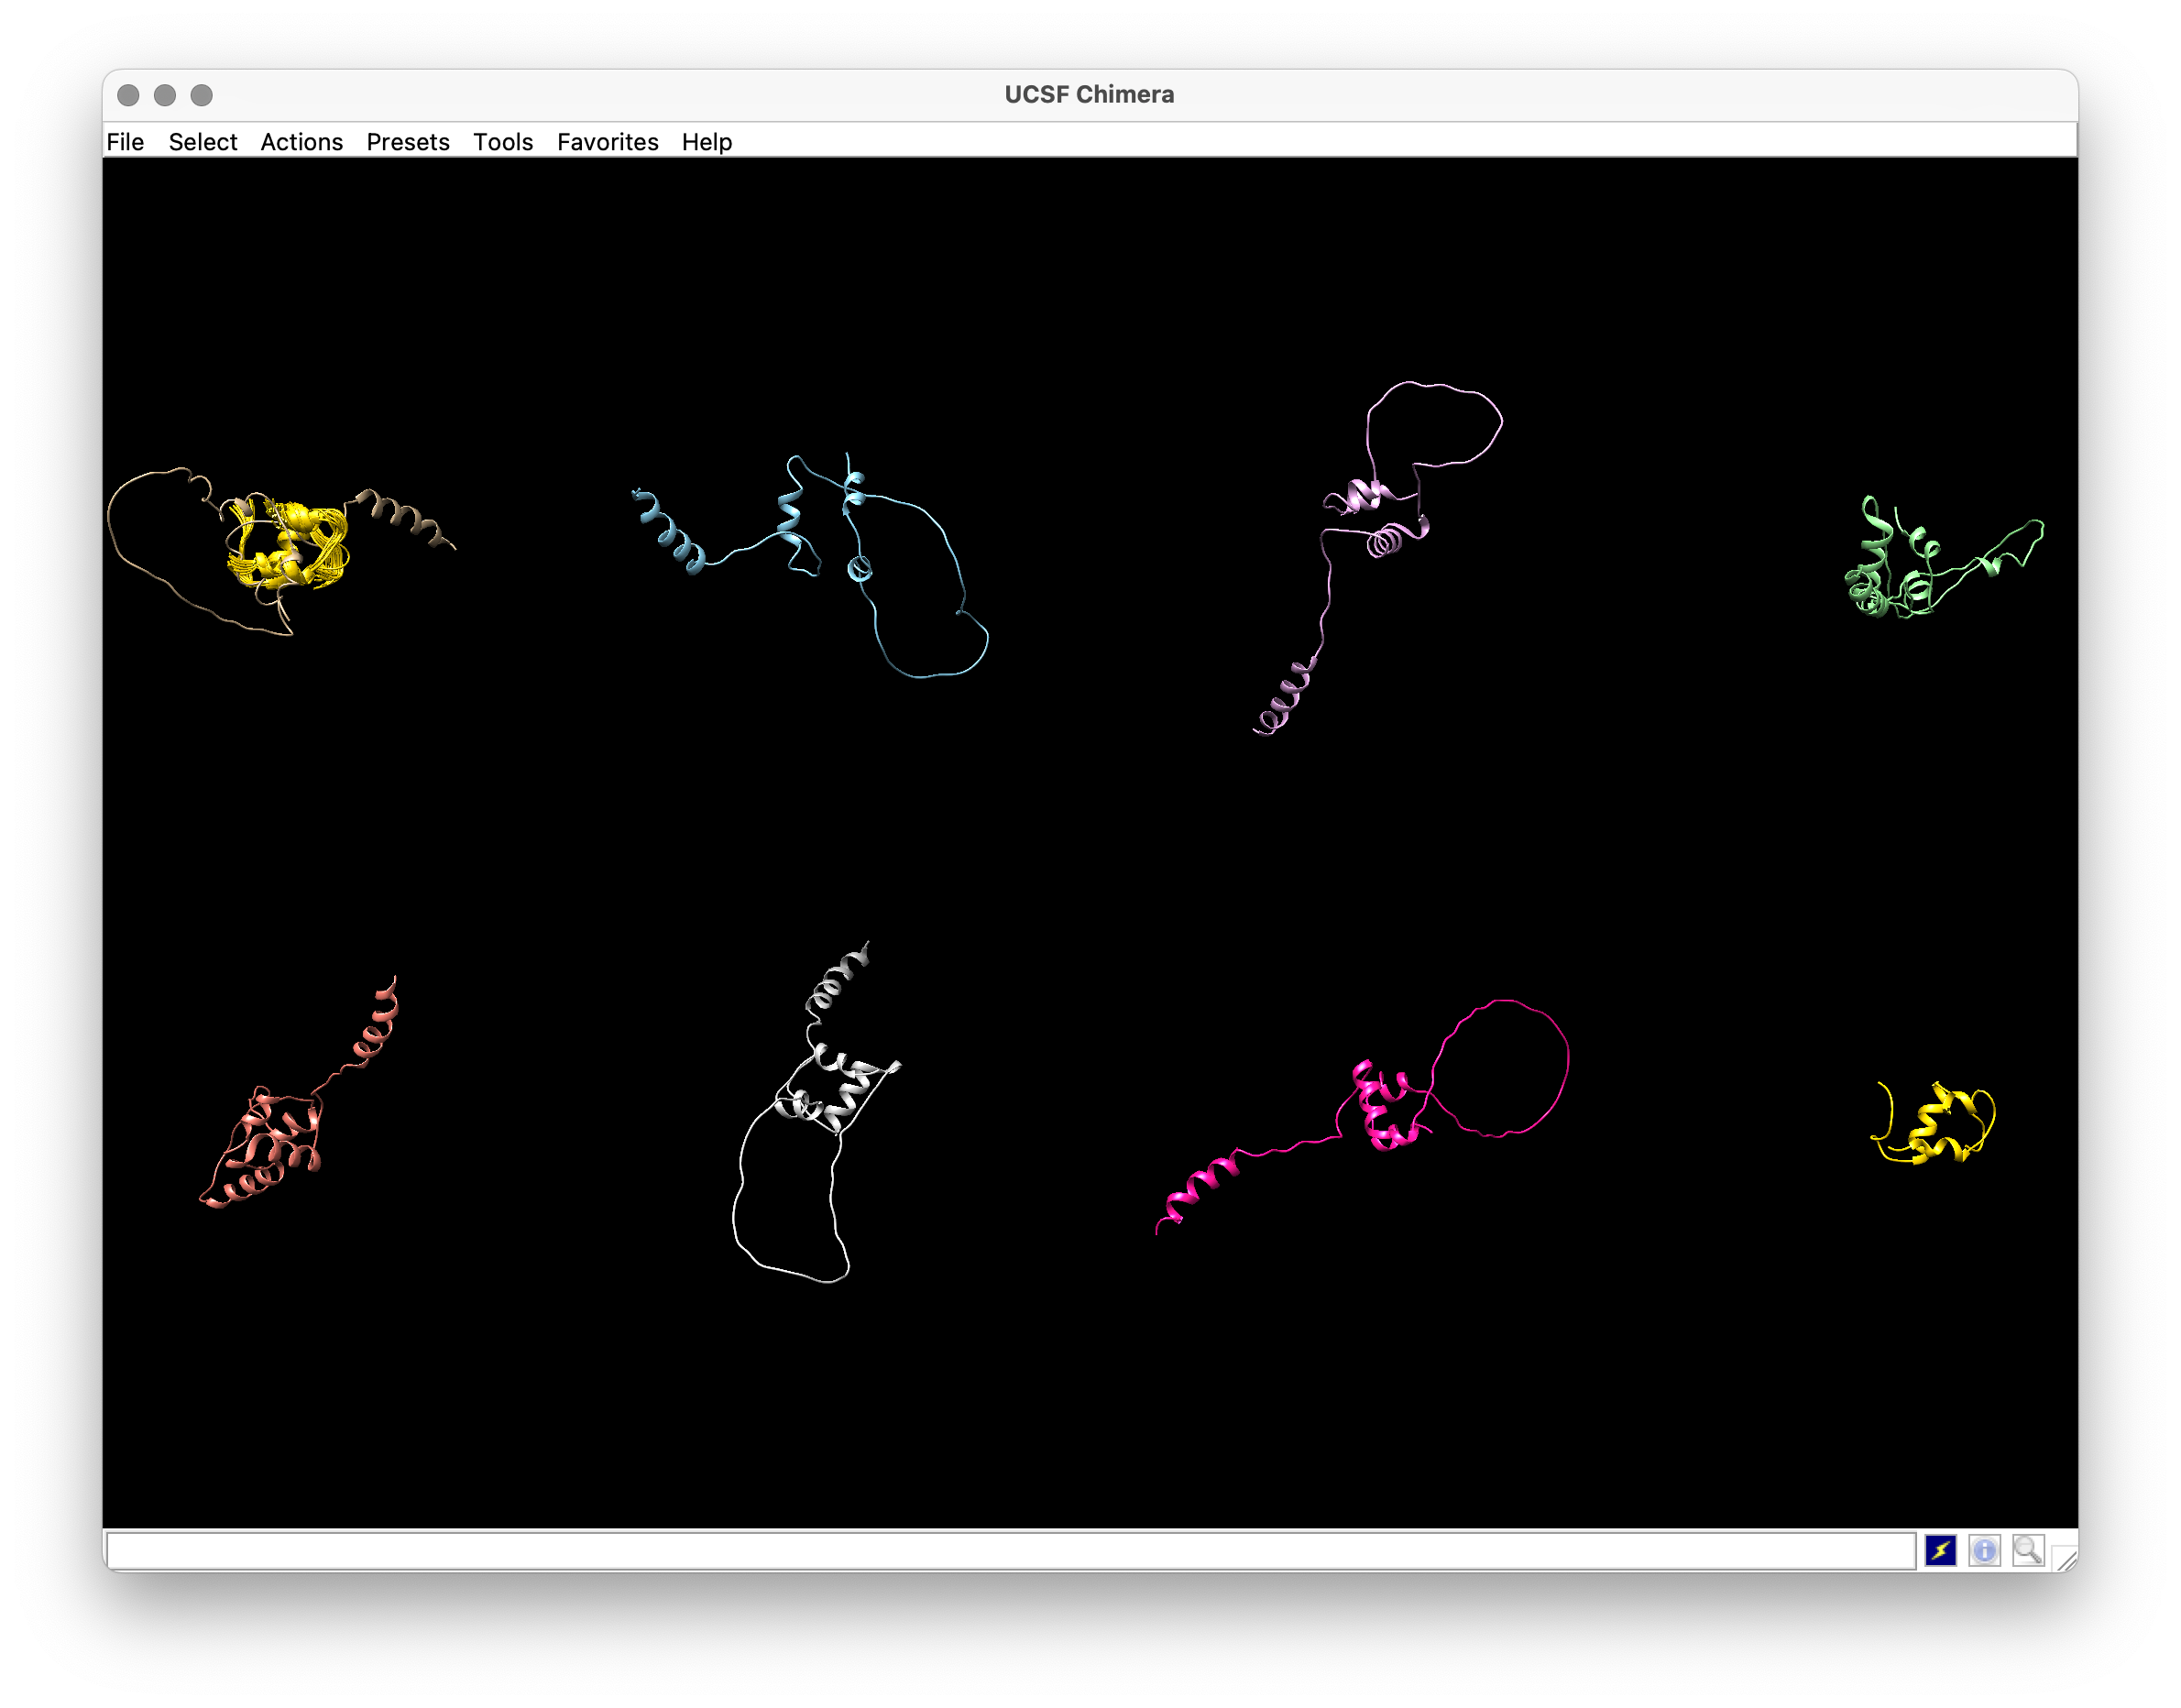
\includegraphics[width=0.8\textwidth]{AAA59172.1/_img/tile}
    \caption{Tiled view of insulin structures from different species showing overall structural conservation.}
    \label{fig:insulin-tile}
\end{figure}

\subsubsection{Structural Alignment}\label{subsubsec:alignment}
The MatchMaker tool was utilized with the following parameters (Figure \ref{fig:matchmaker-settings}):
\begin{itemize}
    \item Alignment algorithm: Needleman-Wunsch
    \item Matrix: BLOSUM-62
    \item Gap opening penalty: 12
    \item Gap extension penalty: 1
    \item Include secondary structure score (30\%)
\end{itemize}

\begin{figure}[H]
    \centering
    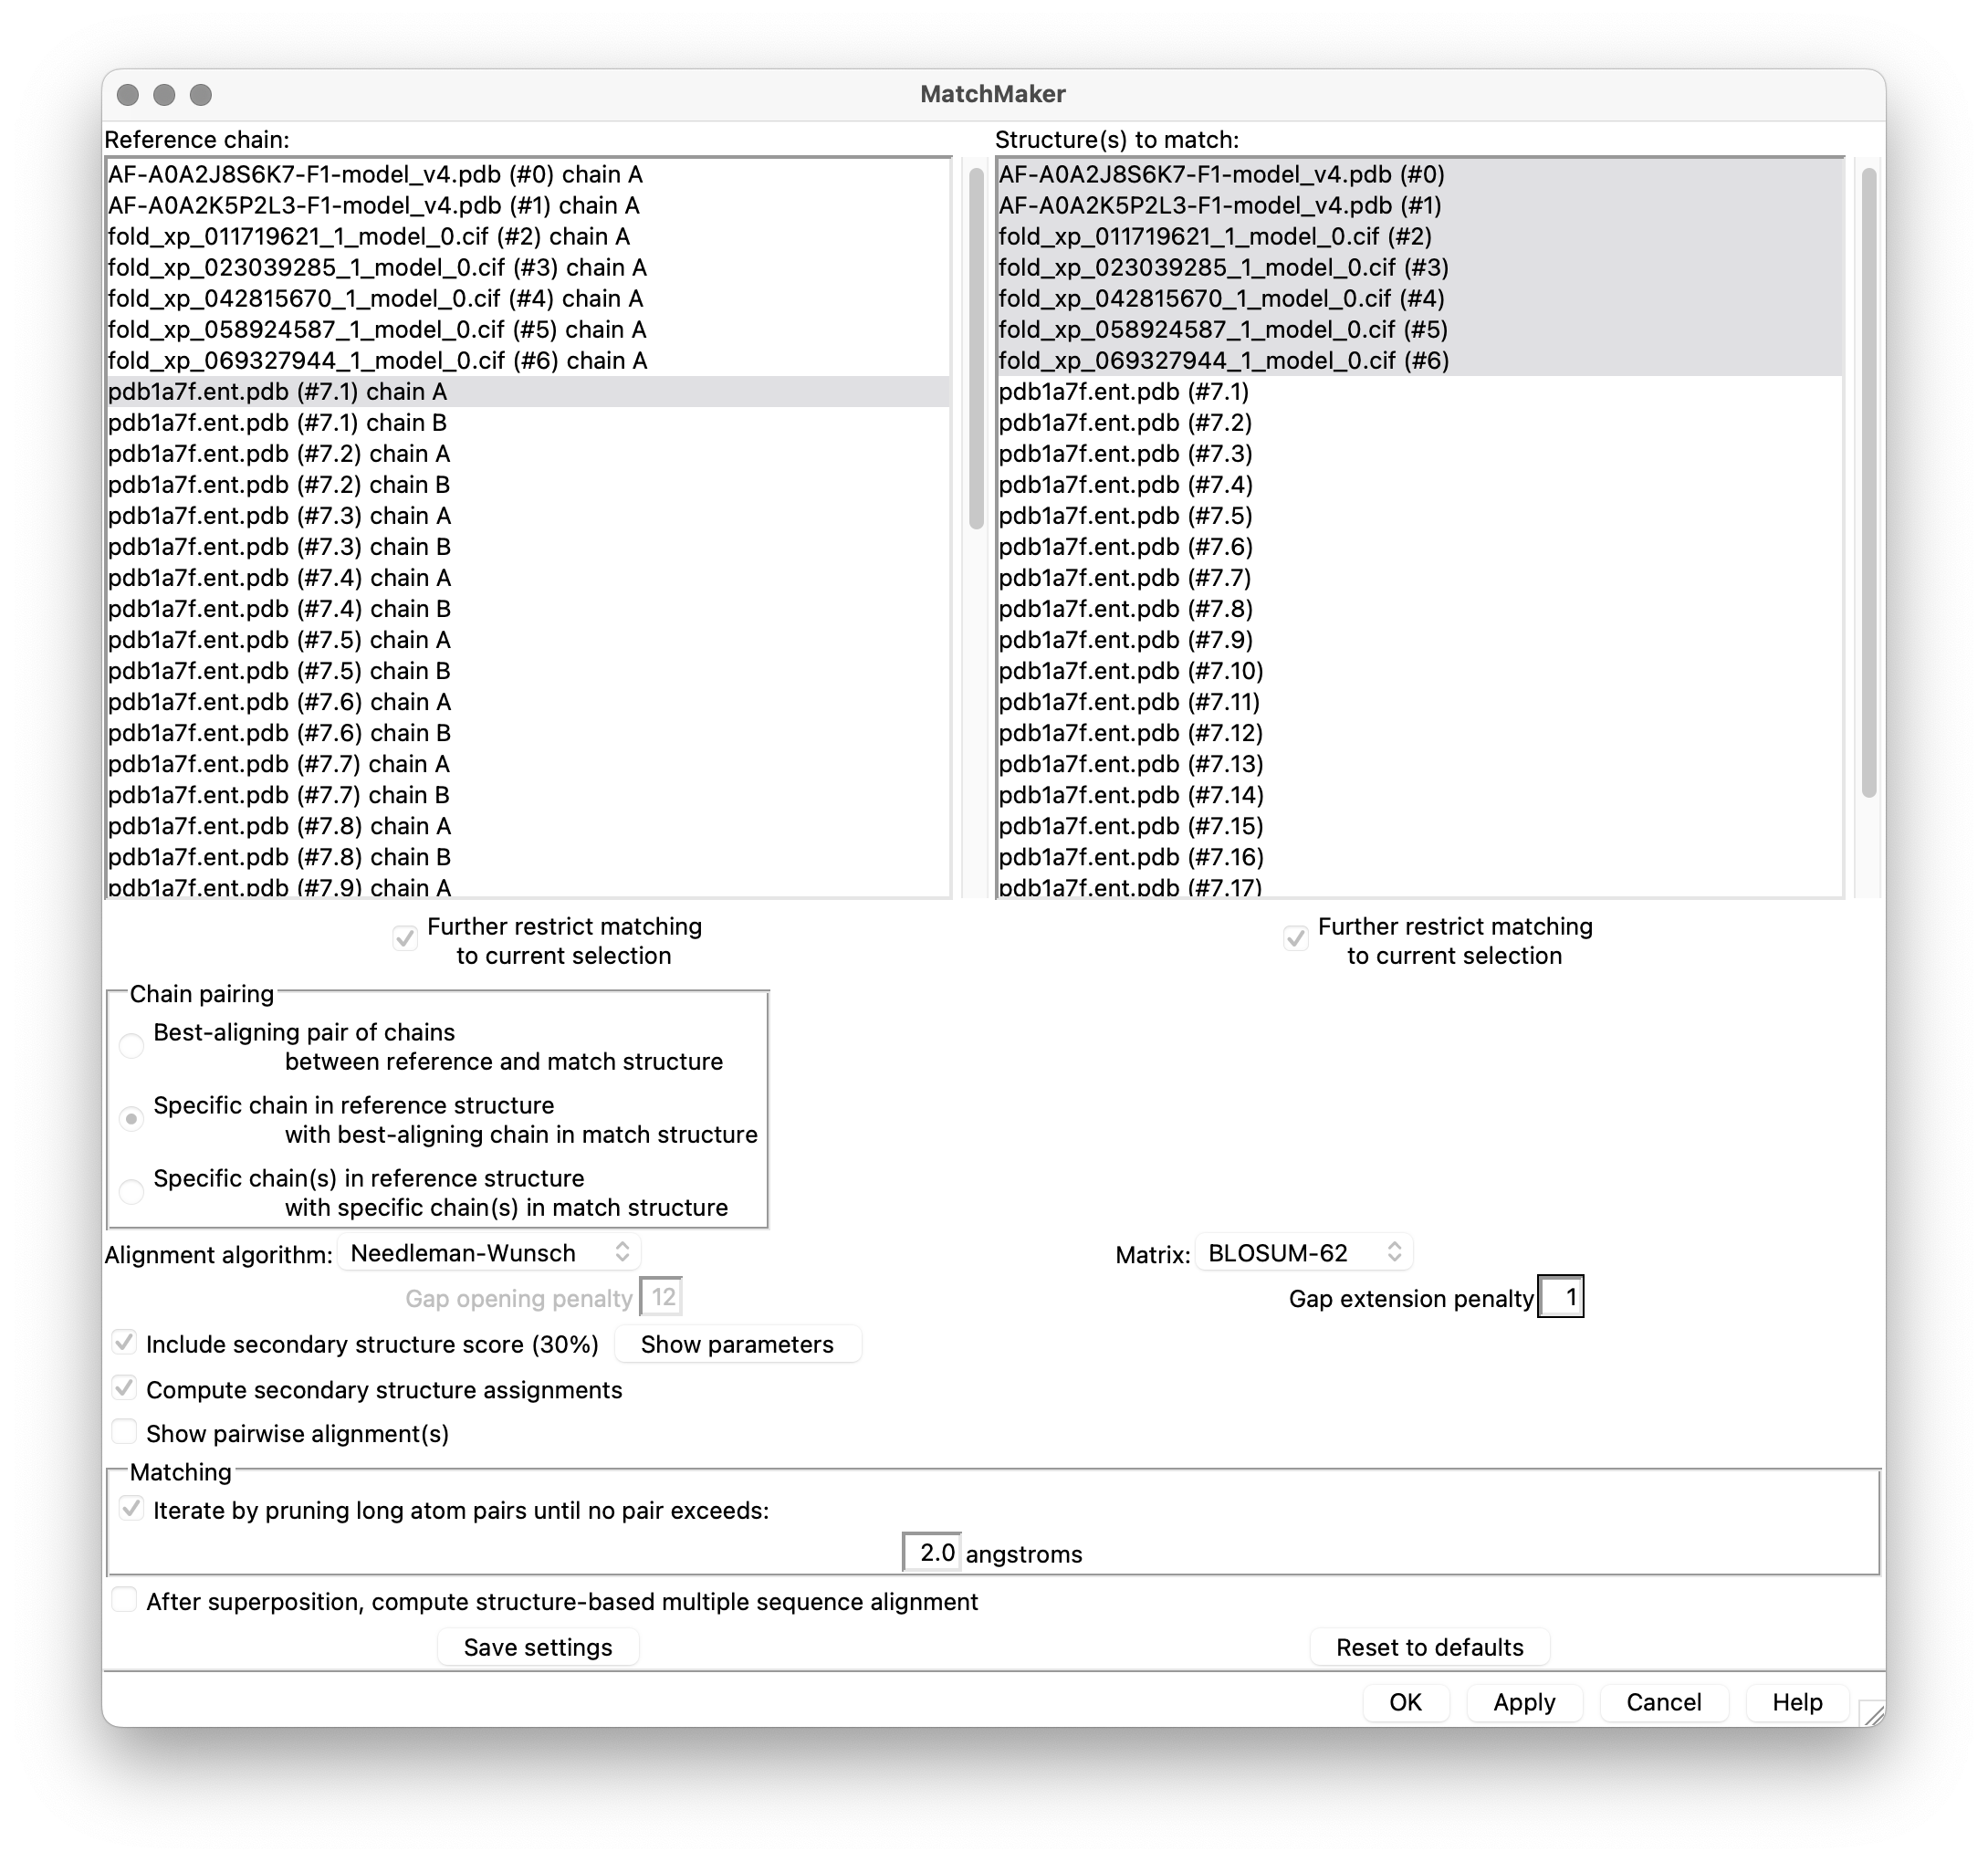
\includegraphics[width=0.8\textwidth]{AAA59172.1/_img/match maker settings}
    \caption{MatchMaker settings used for structural alignment of insulin proteins.}
    \label{fig:matchmaker-settings}
\end{figure}

The structural alignment revealed high conservation among the insulin proteins, with an RMSD of 1.105 angstroms between pruned atom pairs (Figure \ref{fig:alignment-results}). This indicates strong structural preservation across species.

\begin{figure}[H]
    \centering
    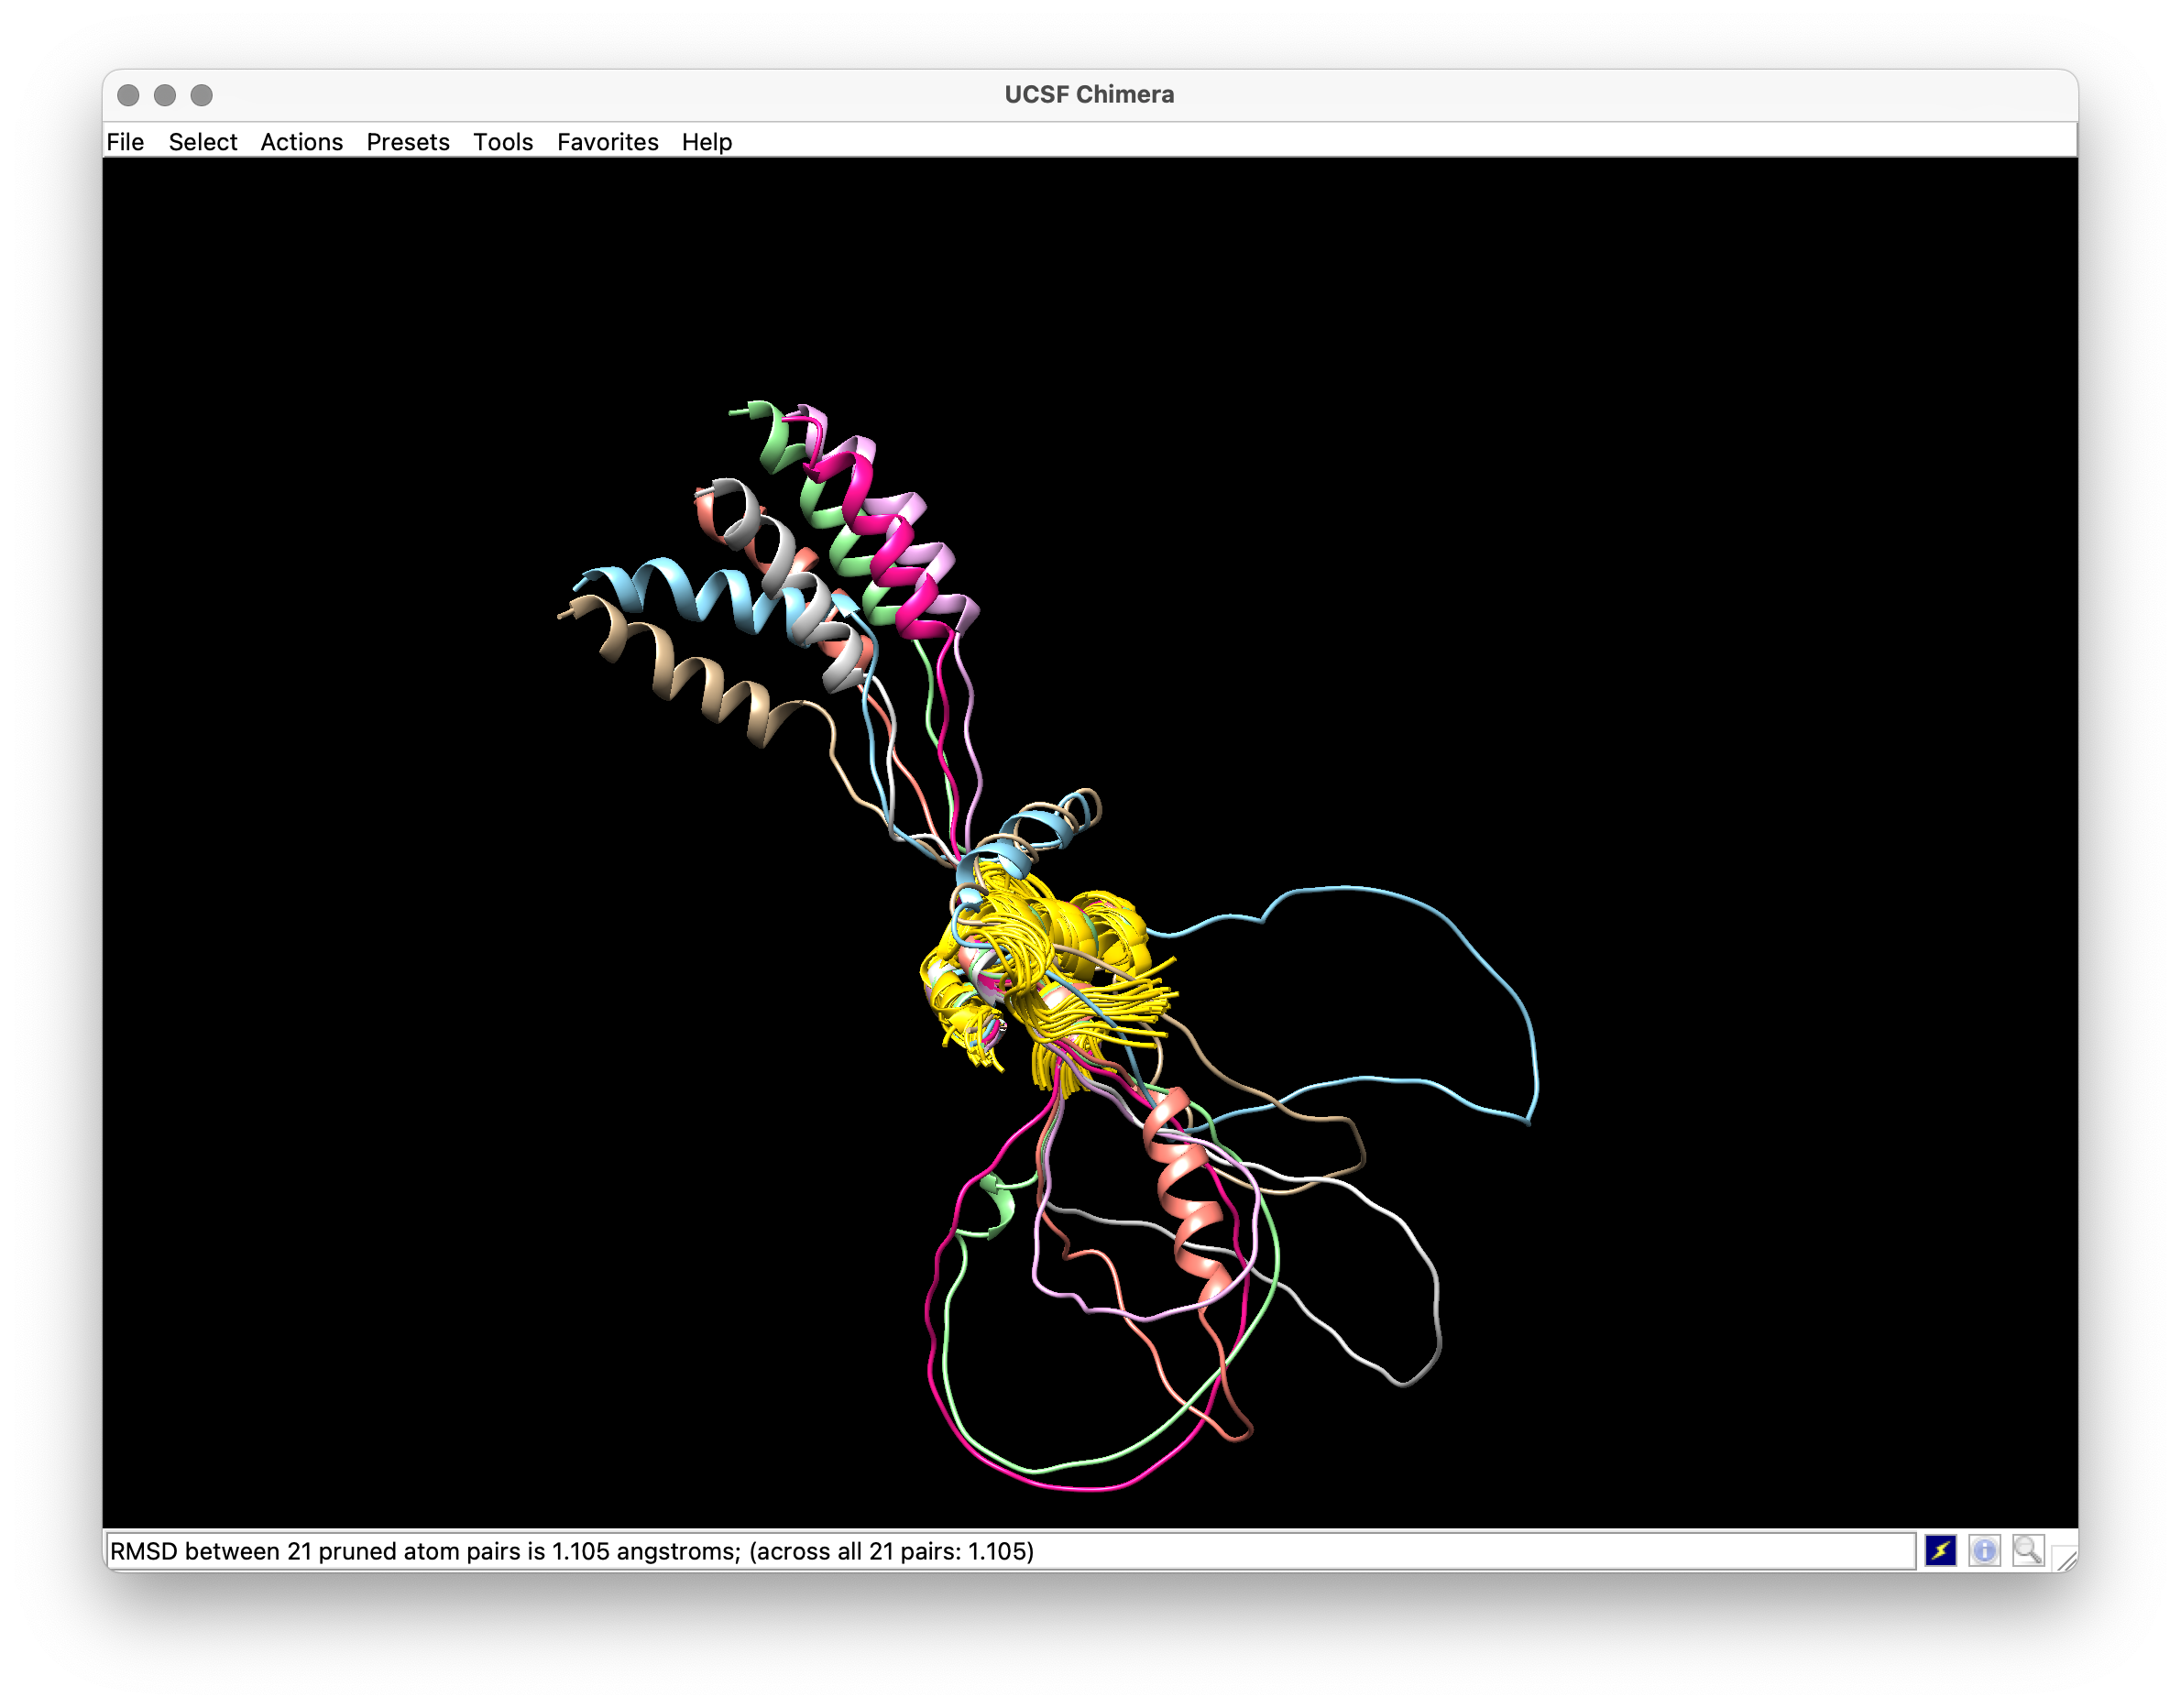
\includegraphics[width=0.8\textwidth]{AAA59172.1/_img/match maker results}
    \caption{Structural alignment results showing superimposed insulin structures.}
    \label{fig:alignment-results}
\end{figure}

\subsubsection{Sequence Conservation Analysis}\label{subsubsec:conservation}
The sequence alignment visualization (Figure \ref{fig:sequence-alignment}) revealed highly conserved regions, particularly in the core structural elements. The sequence identity matrix (Figure \ref{fig:sequence-identity}) showed identity values ranging from 82.57\% to 100\% between different species pairs.

\begin{figure}[H]
    \centering
    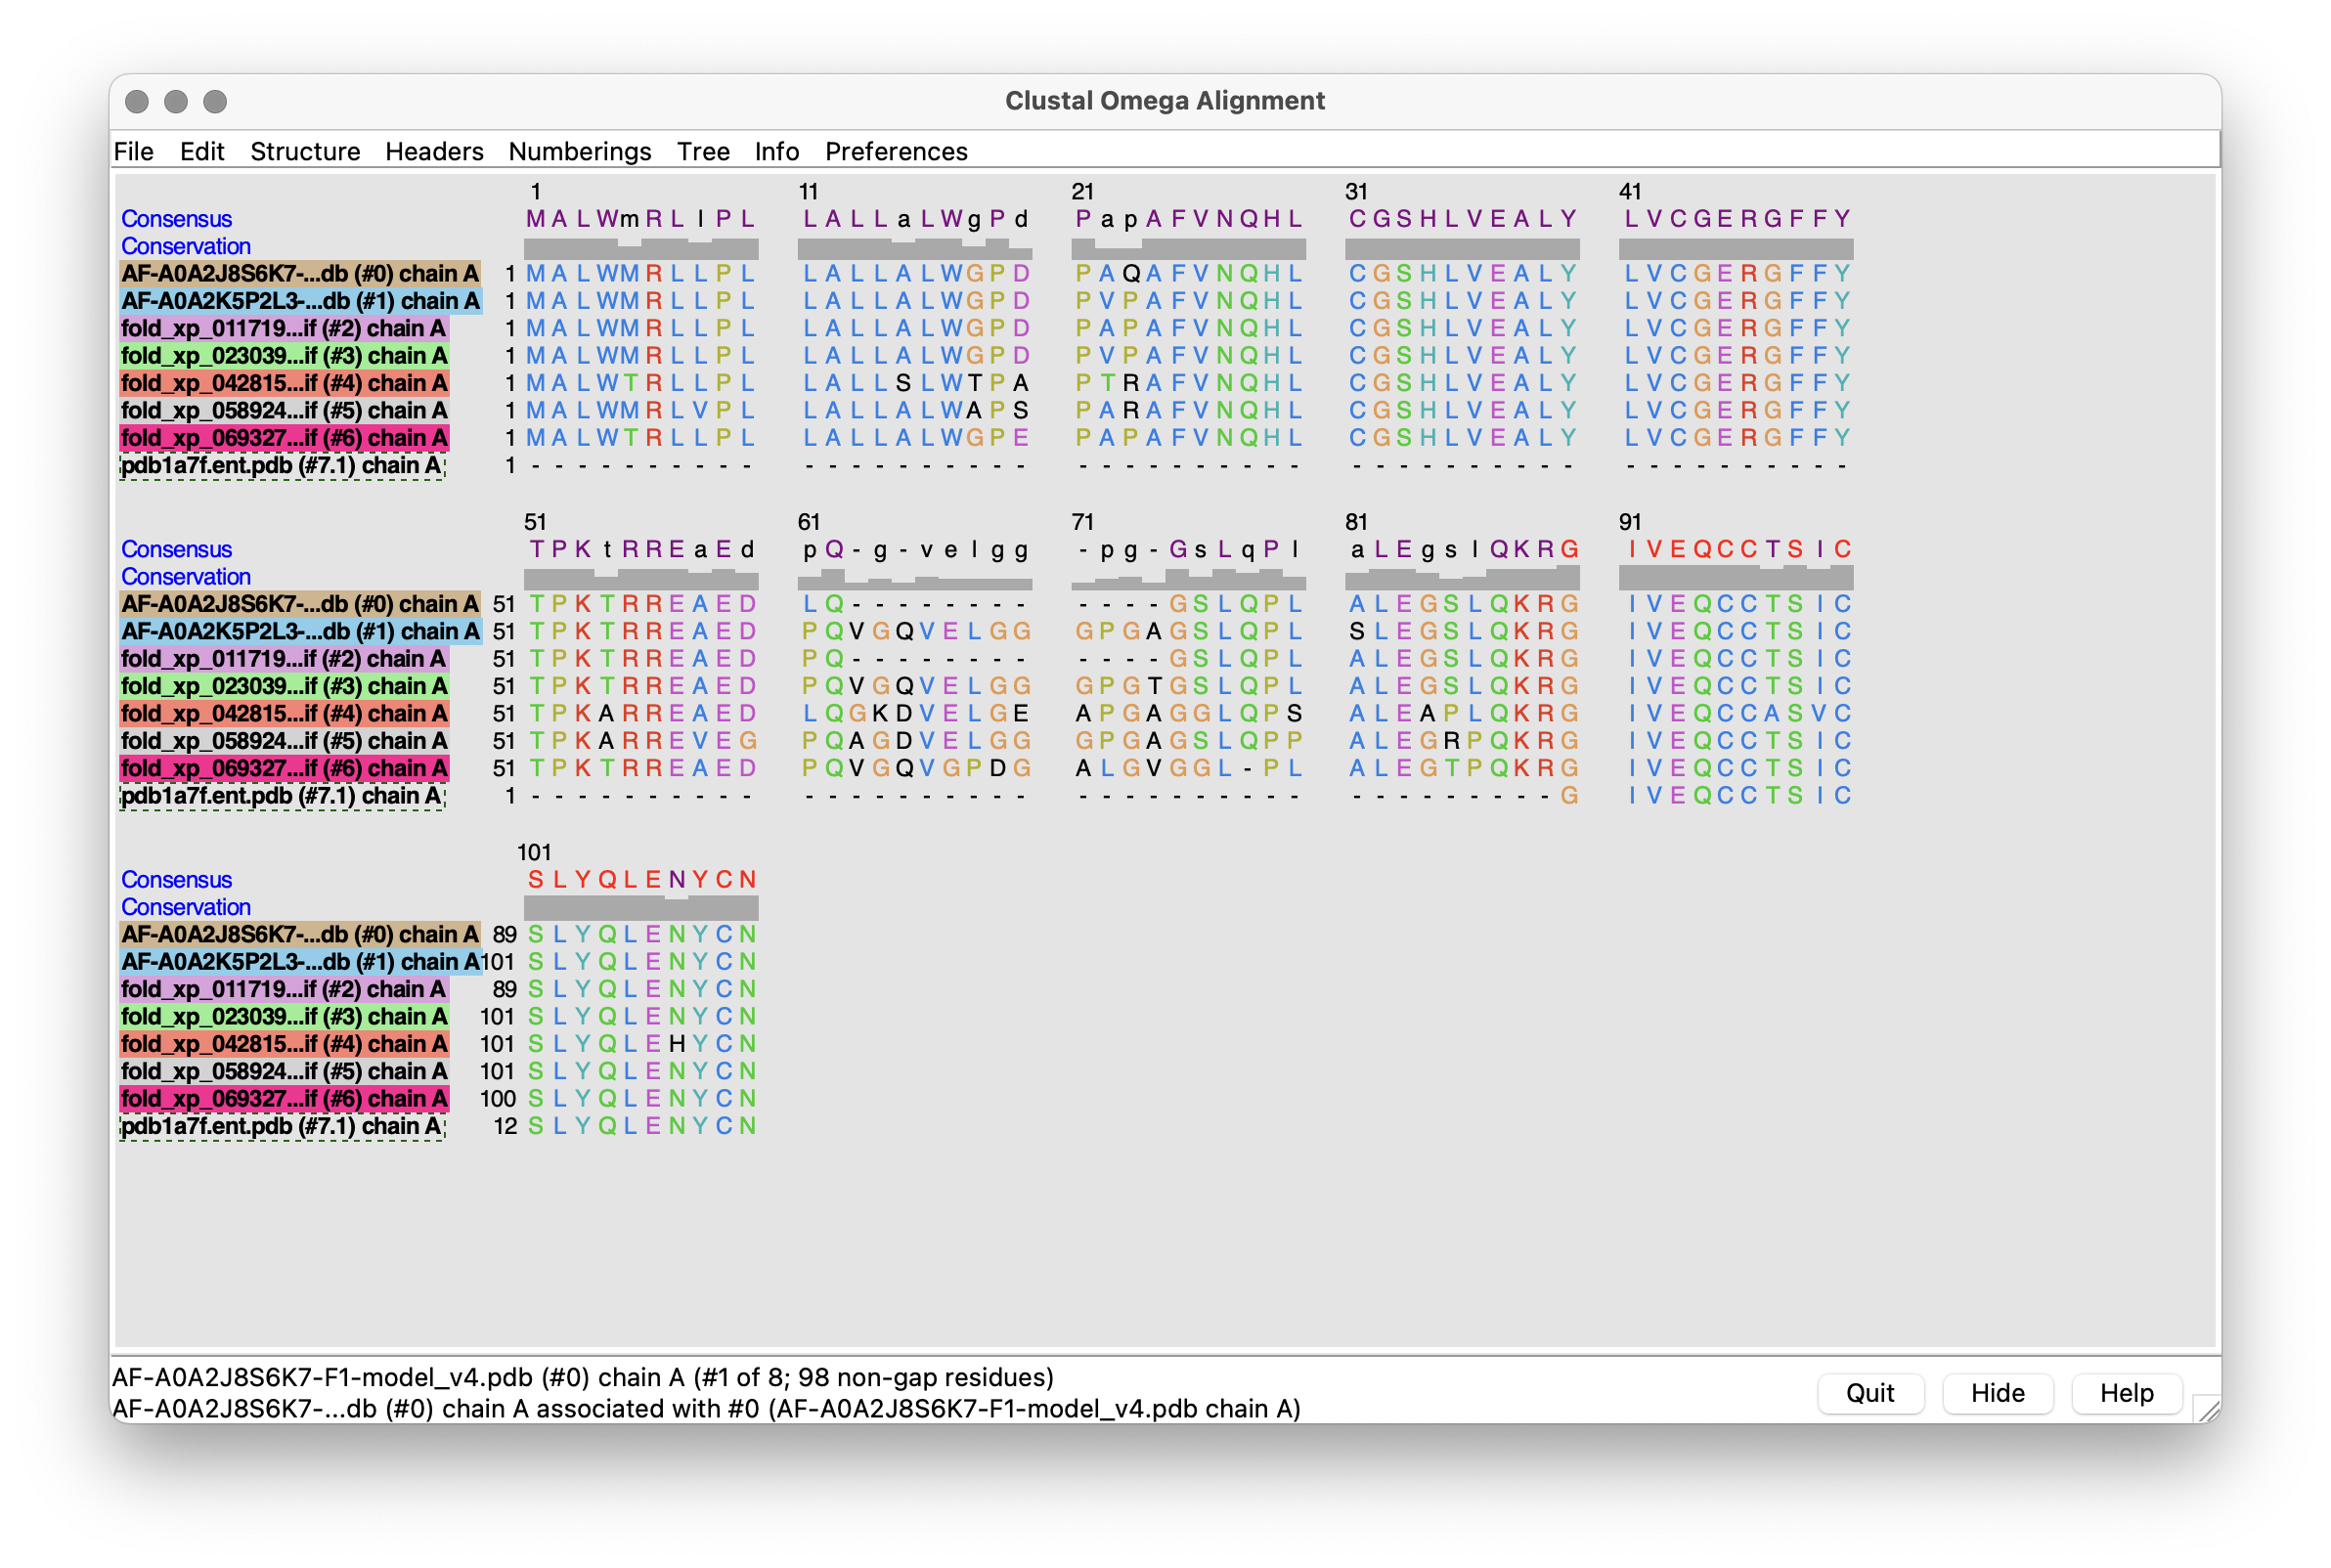
\includegraphics[width=0.8\textwidth]{AAA59172.1/_img/seq alignment results}
    \caption{Multiple sequence alignment of insulin proteins showing conservation patterns.}
    \label{fig:sequence-alignment}
\end{figure}

\begin{figure}[H]
    \centering
    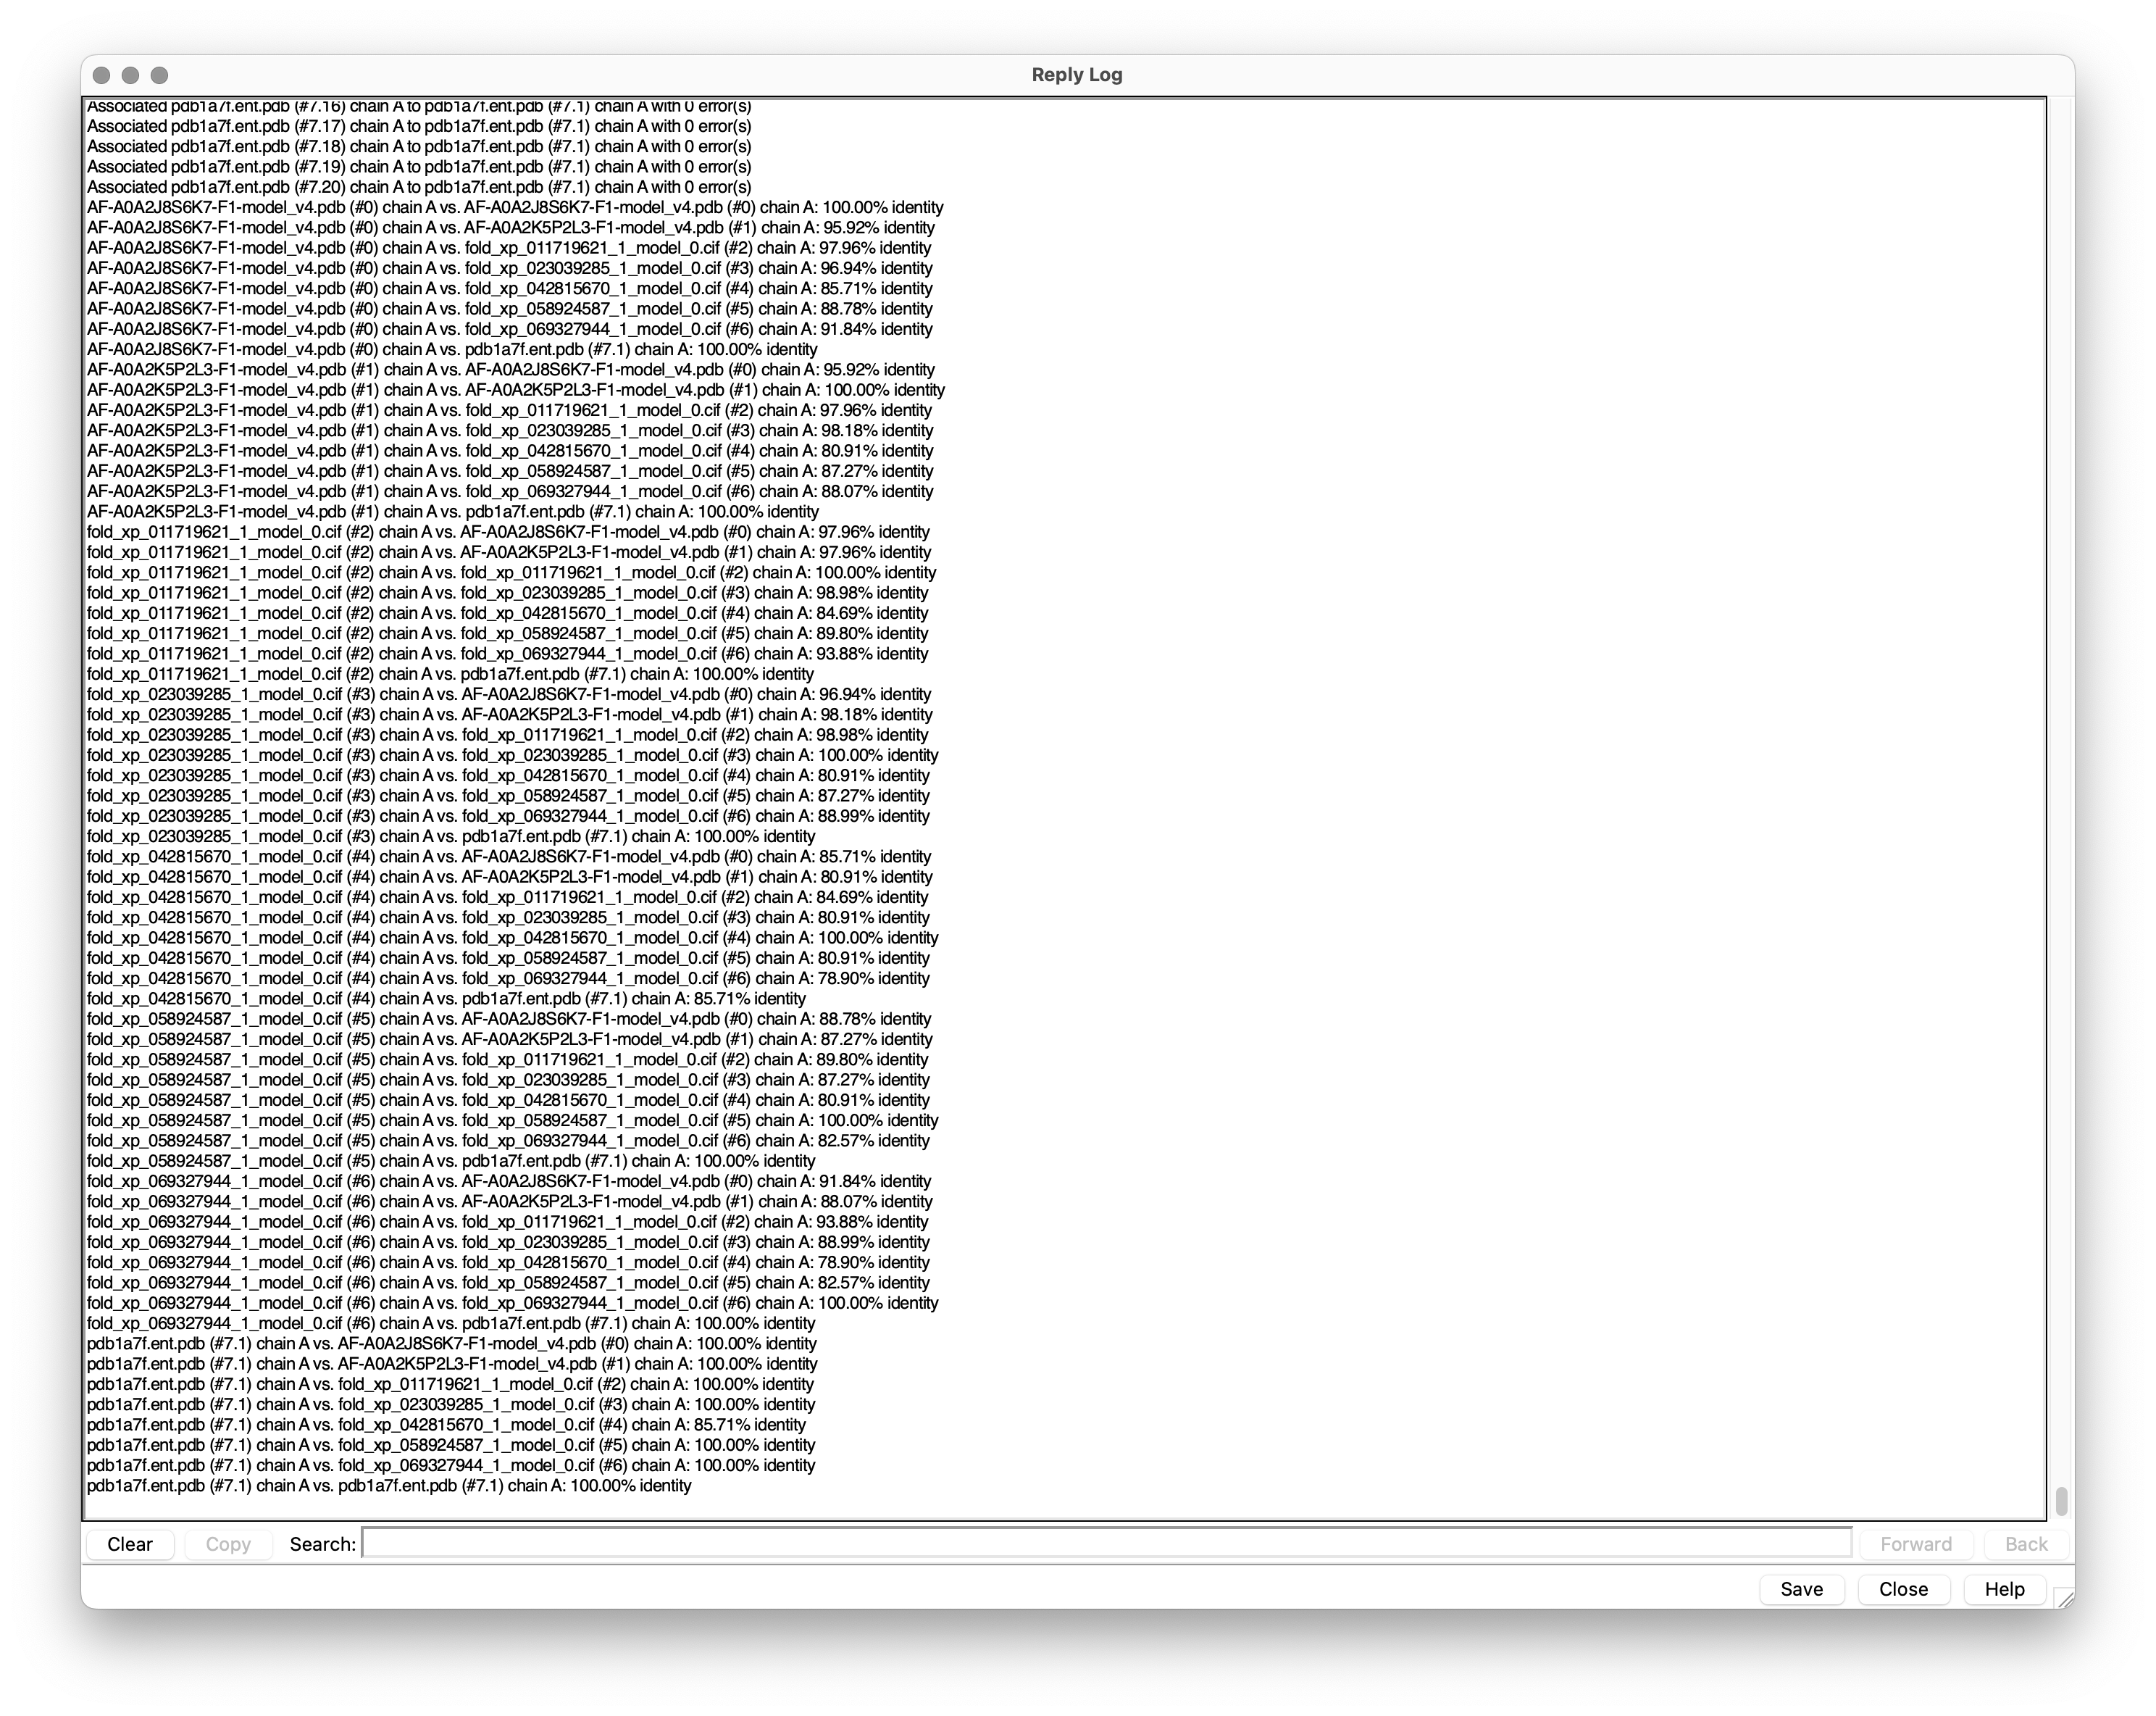
\includegraphics[width=0.8\textwidth]{AAA59172.1/_img/seq identity results}
    \caption{Sequence identity matrix showing pairwise comparisons between insulin structures.}
    \label{fig:sequence-identity}
\end{figure}

\subsubsection{Structure Conservation Visualization}\label{subsubsec:conservation-vis}
The conservation analysis was visualized using Chimera's built-in tools (Figure \ref{fig:conservation-render}), highlighting the structural elements that are most conserved across species.

\begin{figure}[H]
    \centering
    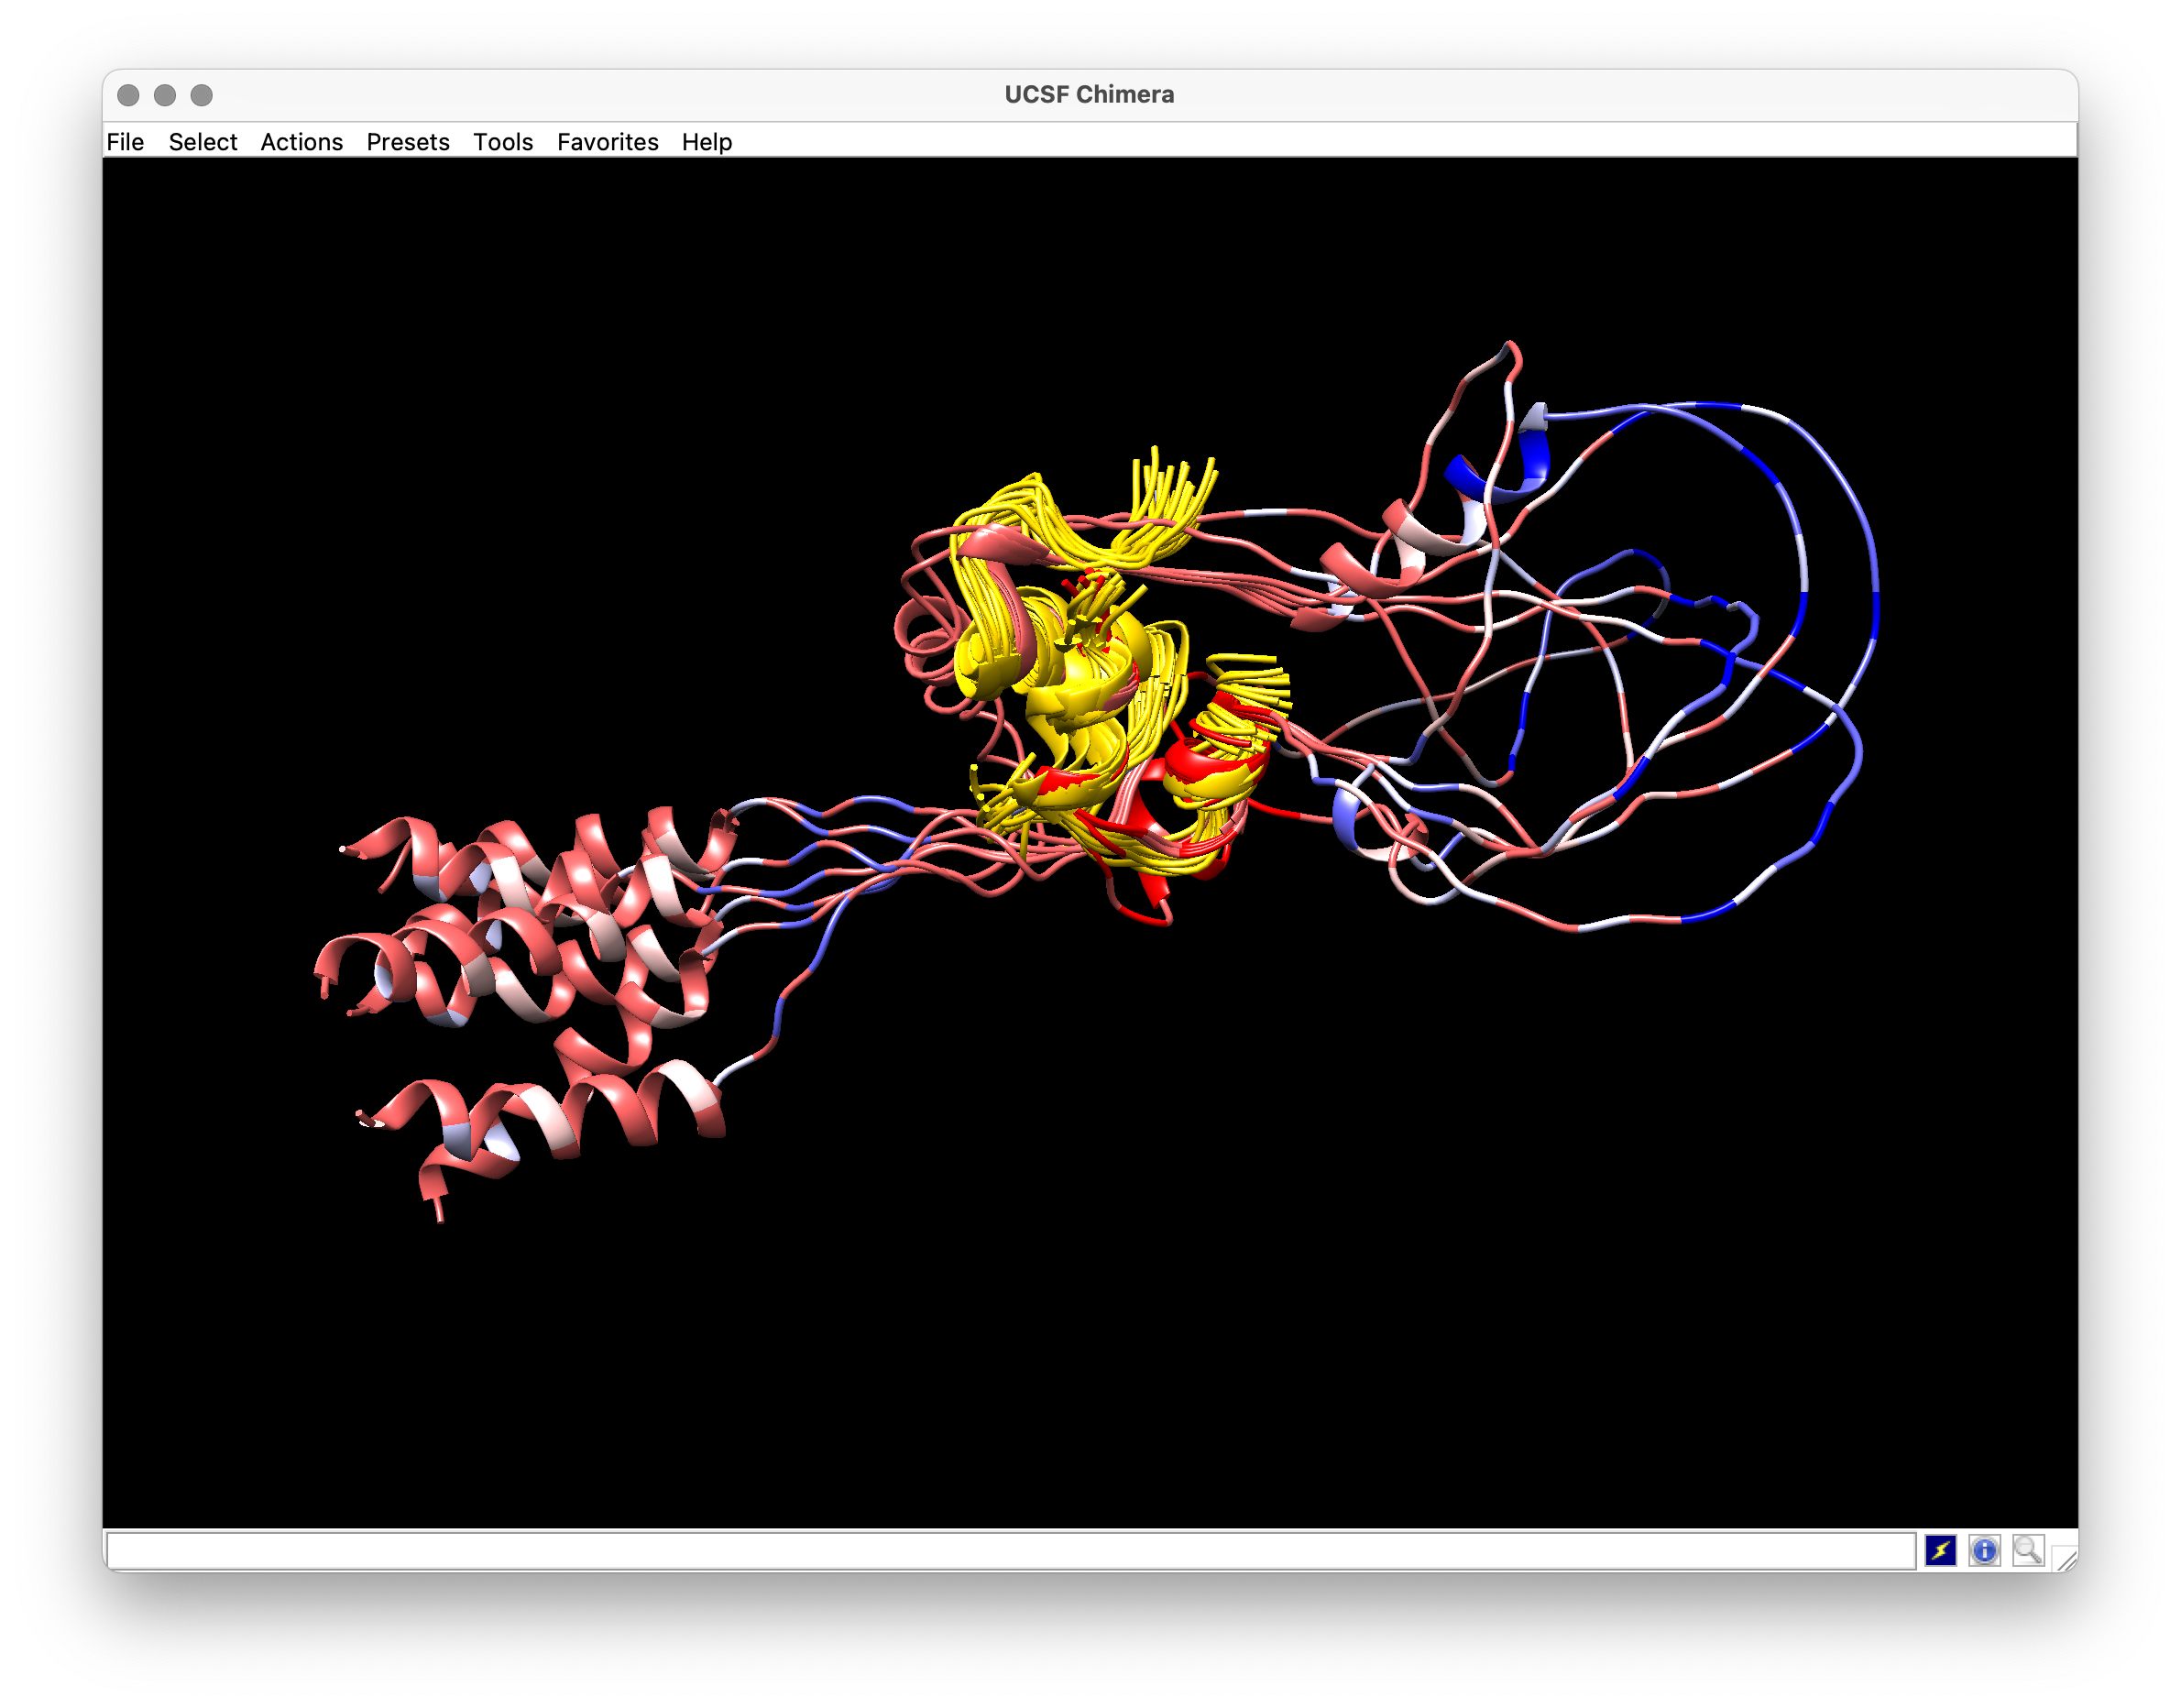
\includegraphics[width=0.8\textwidth]{AAA59172.1/_img/conservation render}
    \caption{Visualization of structural conservation across insulin proteins.}
    \label{fig:conservation-render}
\end{figure}

\subsubsection{Ensemble Analysis}\label{subsubsec:ensemble}
Finally, the Ensemble Match tool was attempted to compare multiple structures simultaneously. However, this resulted in an error due to unequal numbers of atoms in the structures (Figure \ref{fig:ensemble-match}).

\begin{figure}[H]
    \centering
    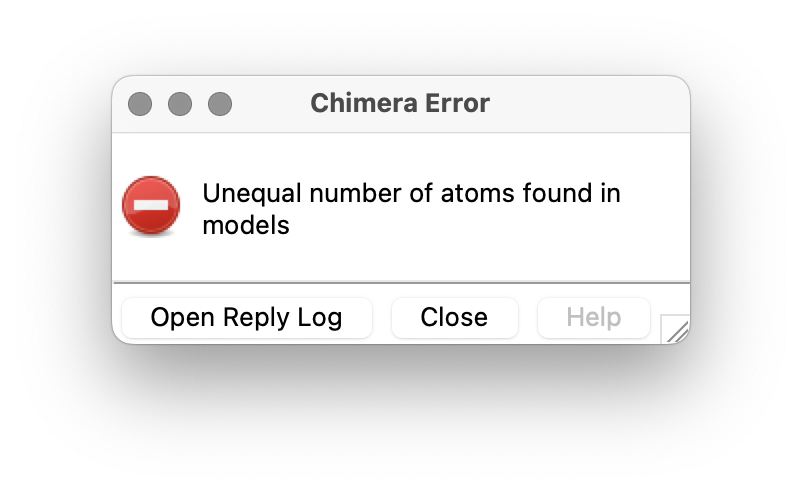
\includegraphics[width=0.8\textwidth]{AAA59172.1/_img/ensemble match}
    \caption{Ensemble Match Gives "Unequal number of atoms" error}
    \label{fig:ensemble-match}
\end{figure}

\subsubsection{Structural Comparison Conclusions}\label{subsubsec:conclusions}

Based on the sequence identity matrix and structural alignment results, the following key observations were made:

\paragraph{Most Similar Structures} The two most similar insulin structures were found between:
\begin{itemize}
    \item Human insulin (pdb1a7f) and fold\_xp\_011719621 (Macaca nemestrina), showing 100\% sequence identity and nearly identical structural alignment
    \item AF-A0A2J8S6K7 (Pongo abelii) and AF-A0A2K5P2L3 (Cercocebus atys), with 95.82\% sequence identity and highly conserved structural elements
\end{itemize}

\paragraph{Most Different Structures} The greatest structural differences were observed between:
\begin{itemize}
    \item fold\_xp\_069327944 (Eulemur rufifrons) and fold\_xp\_058924587 (Kogia breviceps), with 82.57\% sequence identity and notable differences in loop regions
    \item fold\_xp\_042815670 (Panthera tigris) and fold\_xp\_058924587 (Kogia breviceps), showing 87.27\% sequence identity and variations in secondary structure elements
\end{itemize}

\paragraph{Structure-Sequence Correlation} The analysis revealed a strong correlation between sequence differences and structural variations:
\begin{itemize}
    \item Regions with high sequence conservation ($>$95\% identity) showed minimal structural deviation (RMSD $<$ 1.0\AA)
    \item The majority of structural differences were located in loop regions, which also showed lower sequence conservation
    \item Secondary structure elements (alpha-helices and beta-sheets) remained highly conserved even in species pairs with lower sequence identity
    \item The overall fold topology was maintained across all species, despite local variations in less conserved regions
\end{itemize}

These findings demonstrate that sequence differences do correlate well with structural variations, particularly in the flexible regions of the protein. However, the core structural elements of insulin remain highly conserved across species, reflecting the functional importance of these regions.

\subsection{Analysis of Histamine Structures}\label{subsec:histamine-analysis}

The structural analysis of the histamine protein group was conducted using UCSF Chimera, following several key steps:

\subsubsection{Initial Visualization}\label{subsubsec:histamine-visualization}
All histamine structures were loaded and visualized simultaneously using Chimera's tile function (Figure \ref{fig:histamine-tile}). This initial visualization revealed the general structural characteristics of histamine across different species, showing a predominantly helical structure with connecting loops.

\begin{figure}[H]
    \centering
    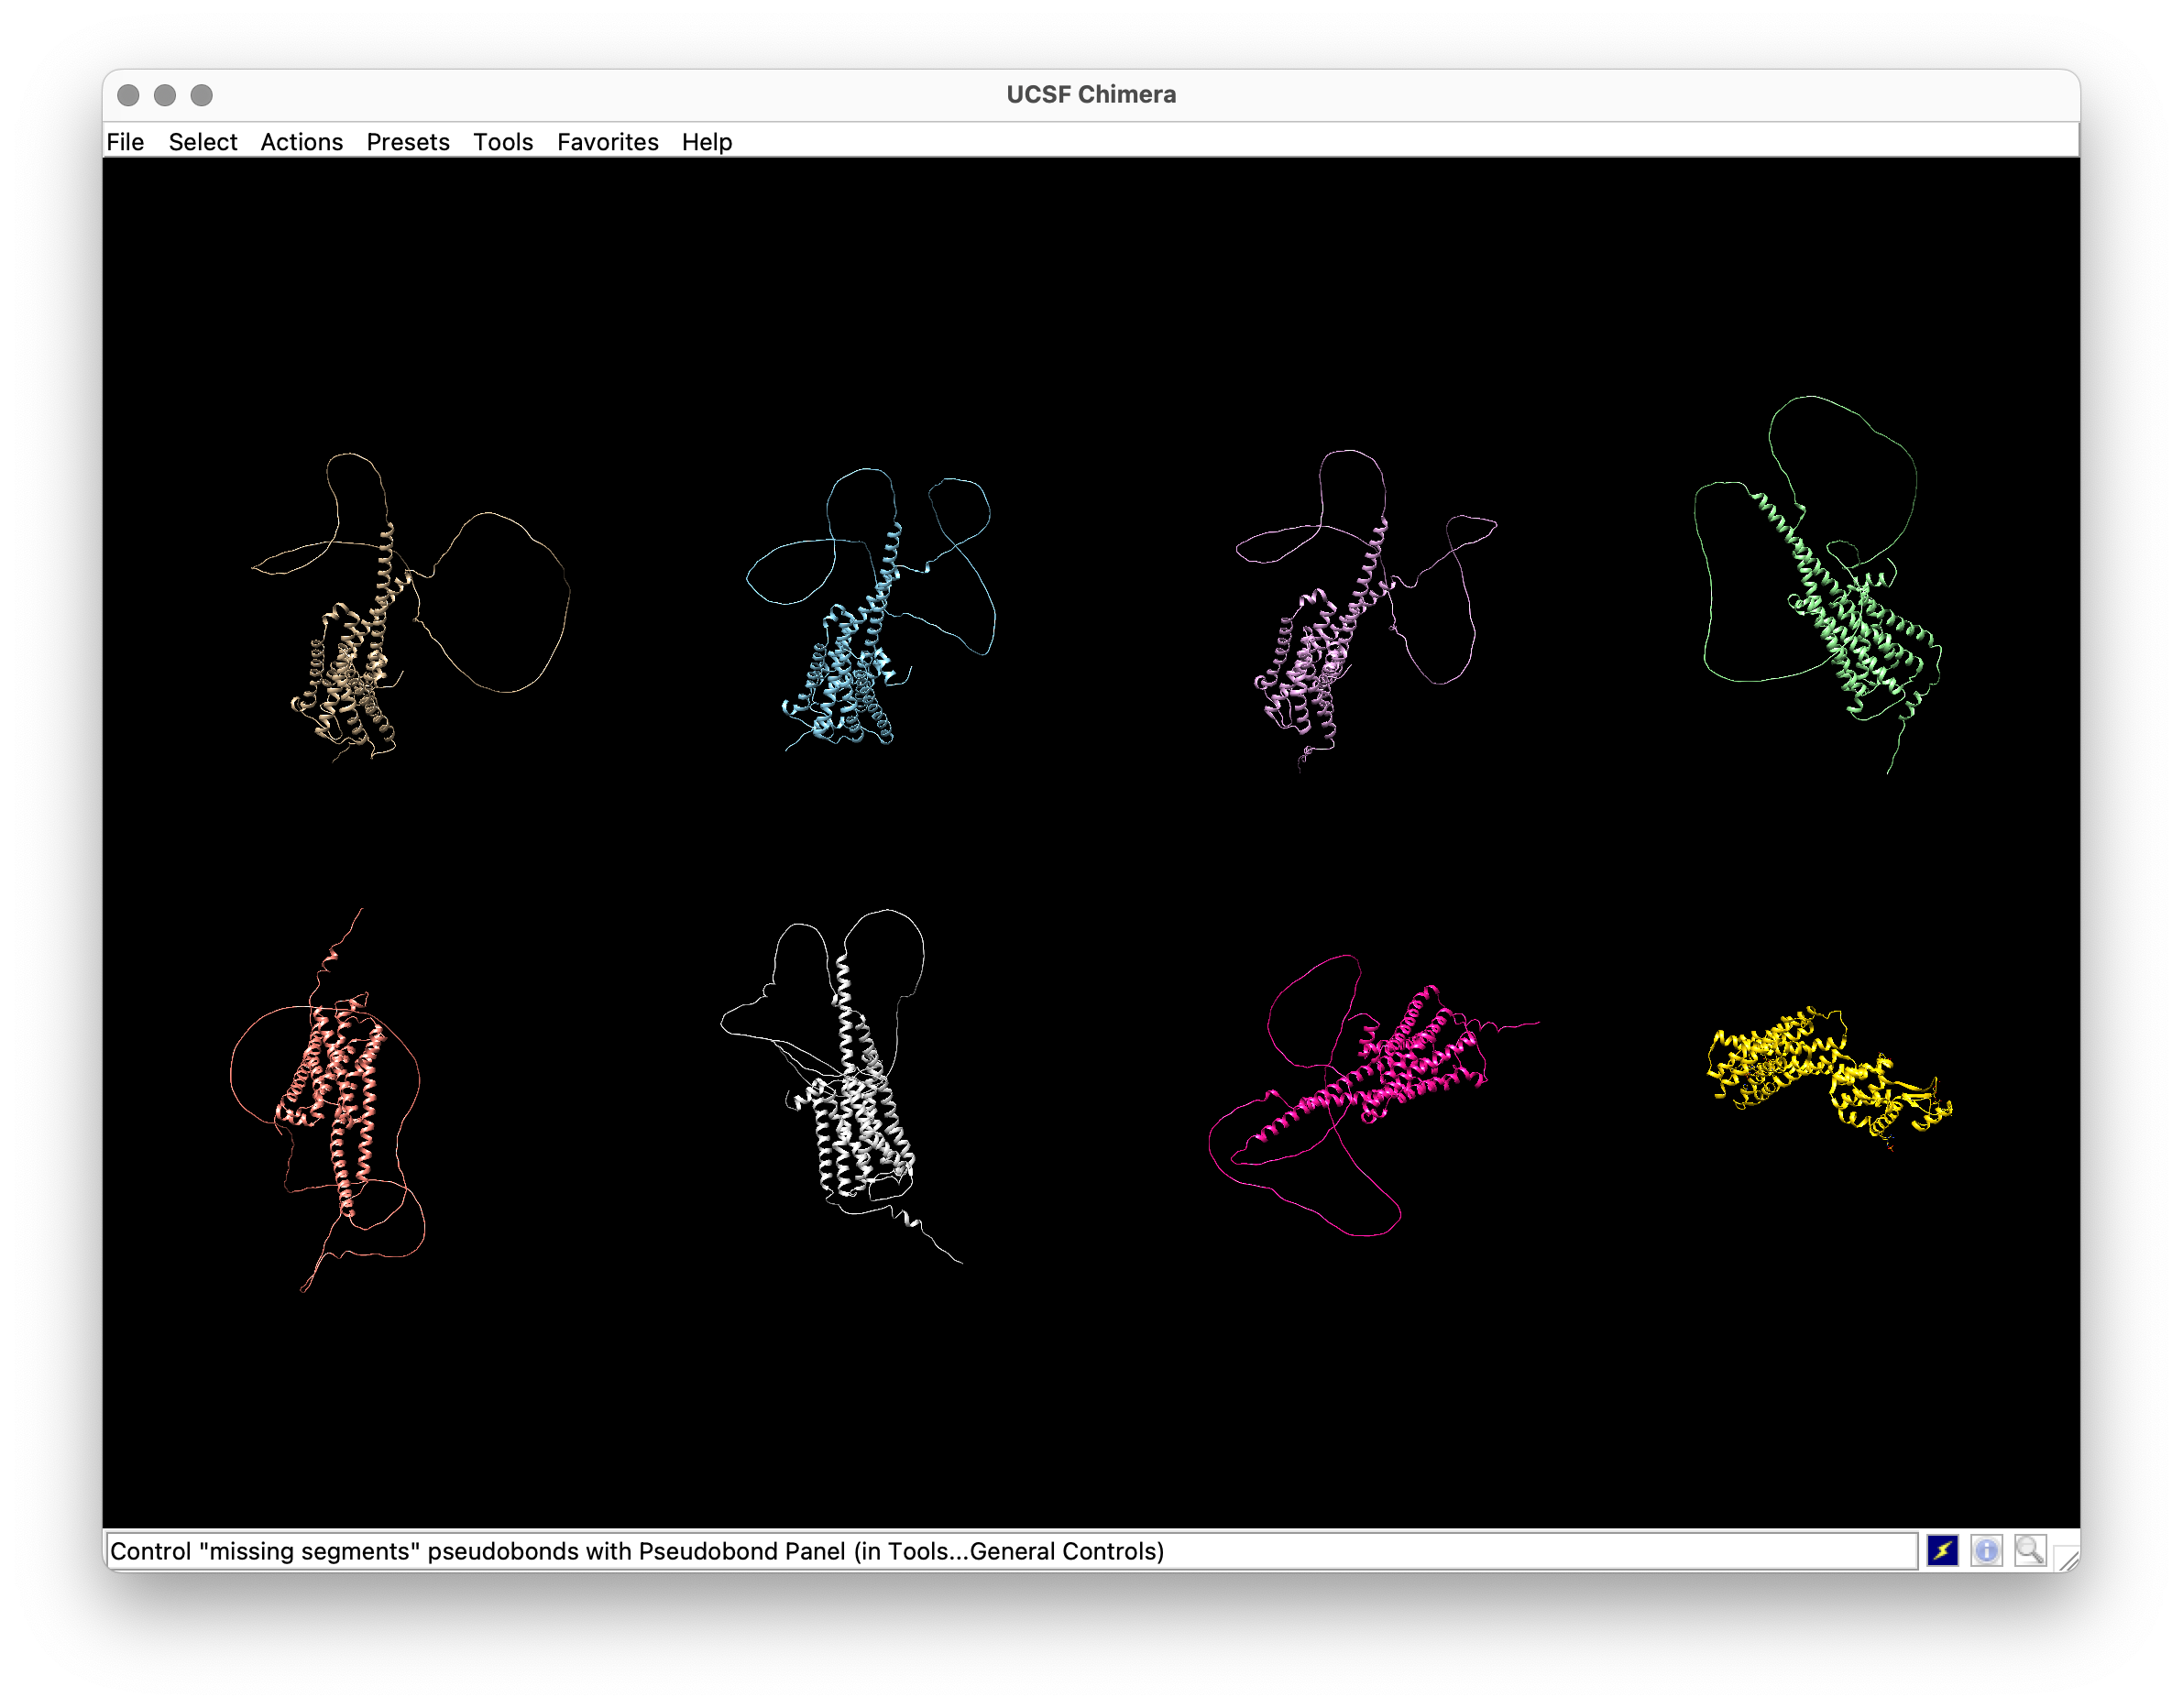
\includegraphics[width=0.8\textwidth]{CAA84380.1/_img/tile}
    \caption{Tiled view of histamine structures from different species showing overall structural conservation.}
    \label{fig:histamine-tile}
\end{figure}

\subsubsection{Structural Alignment}\label{subsubsec:histamine-alignment}
The MatchMaker tool was utilized with the following parameters (Figure \ref{fig:histamine-matchmaker-settings}):
\begin{itemize}
    \item Alignment algorithm: Needleman-Wunsch
    \item Matrix: BLOSUM-62
    \item Gap opening penalty: 12
    \item Gap extension penalty: 1
    \item Include secondary structure score (30\%)
\end{itemize}

\begin{figure}[H]
    \centering
    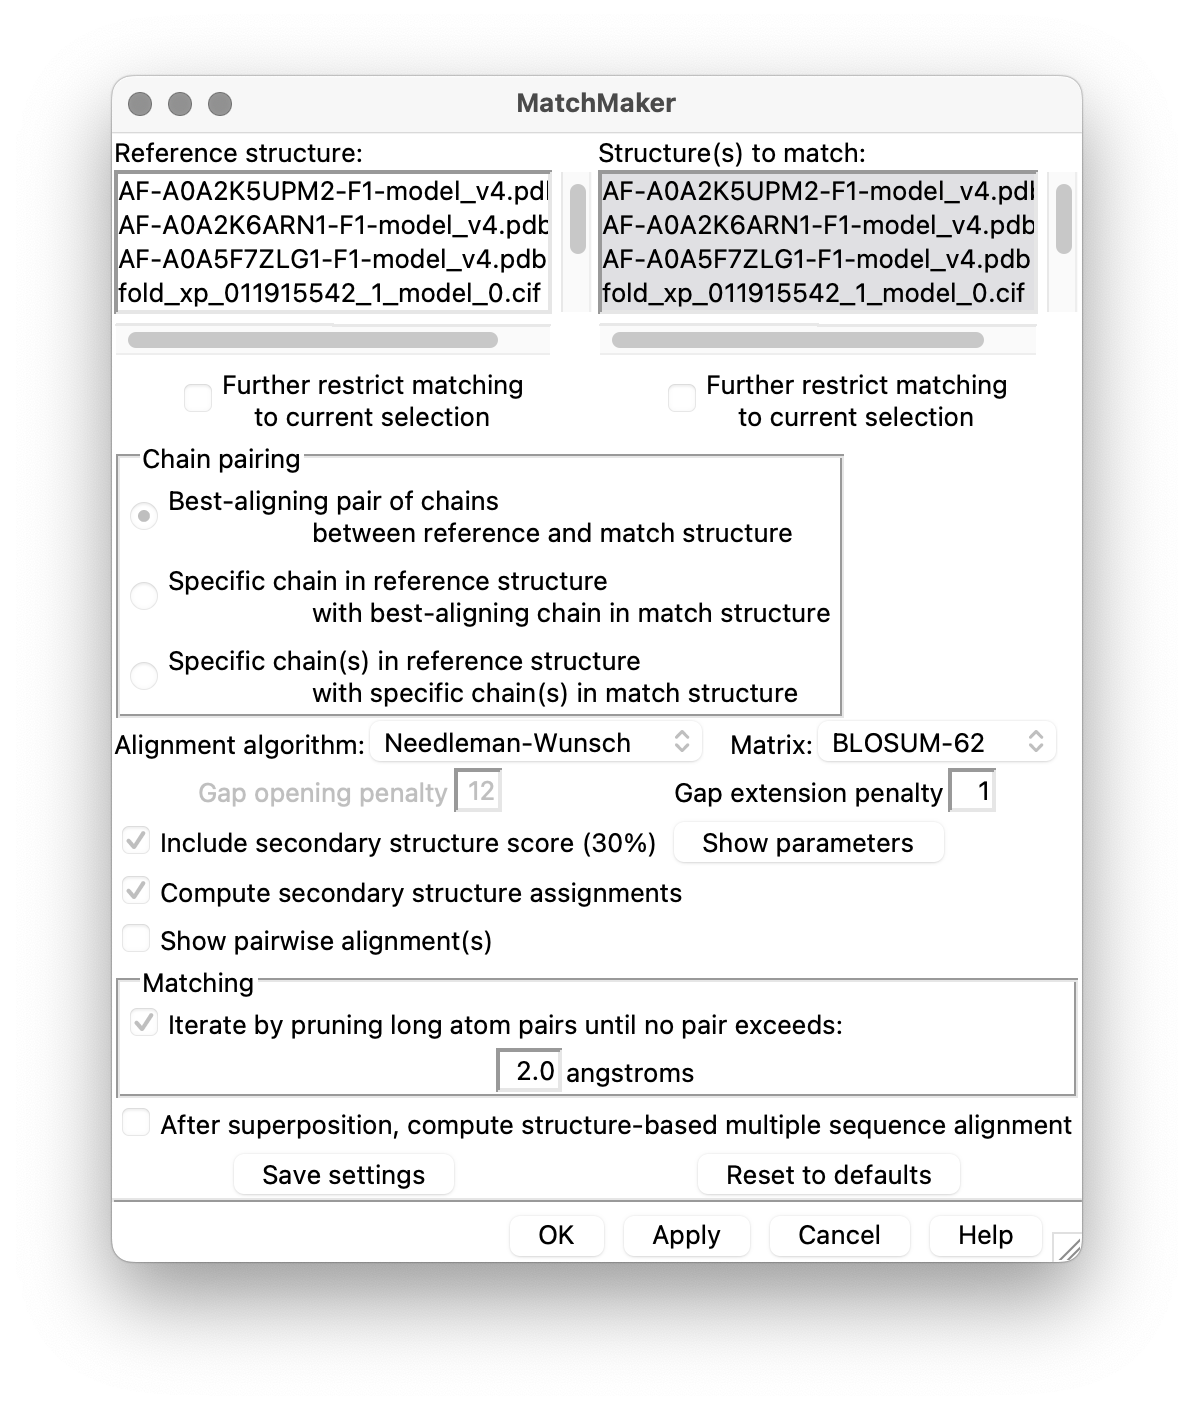
\includegraphics[width=0.8\textwidth]{CAA84380.1/_img/match maker settings}
    \caption{MatchMaker settings used for structural alignment of histamine proteins.}
    \label{fig:histamine-matchmaker-settings}
\end{figure}

The structural alignment revealed high conservation among the histamine proteins, with an RMSD of 0.940 angstroms between pruned atom pairs (Figure \ref{fig:histamine-alignment-results}). This indicates strong structural preservation across species.

\begin{figure}[H]
    \centering
    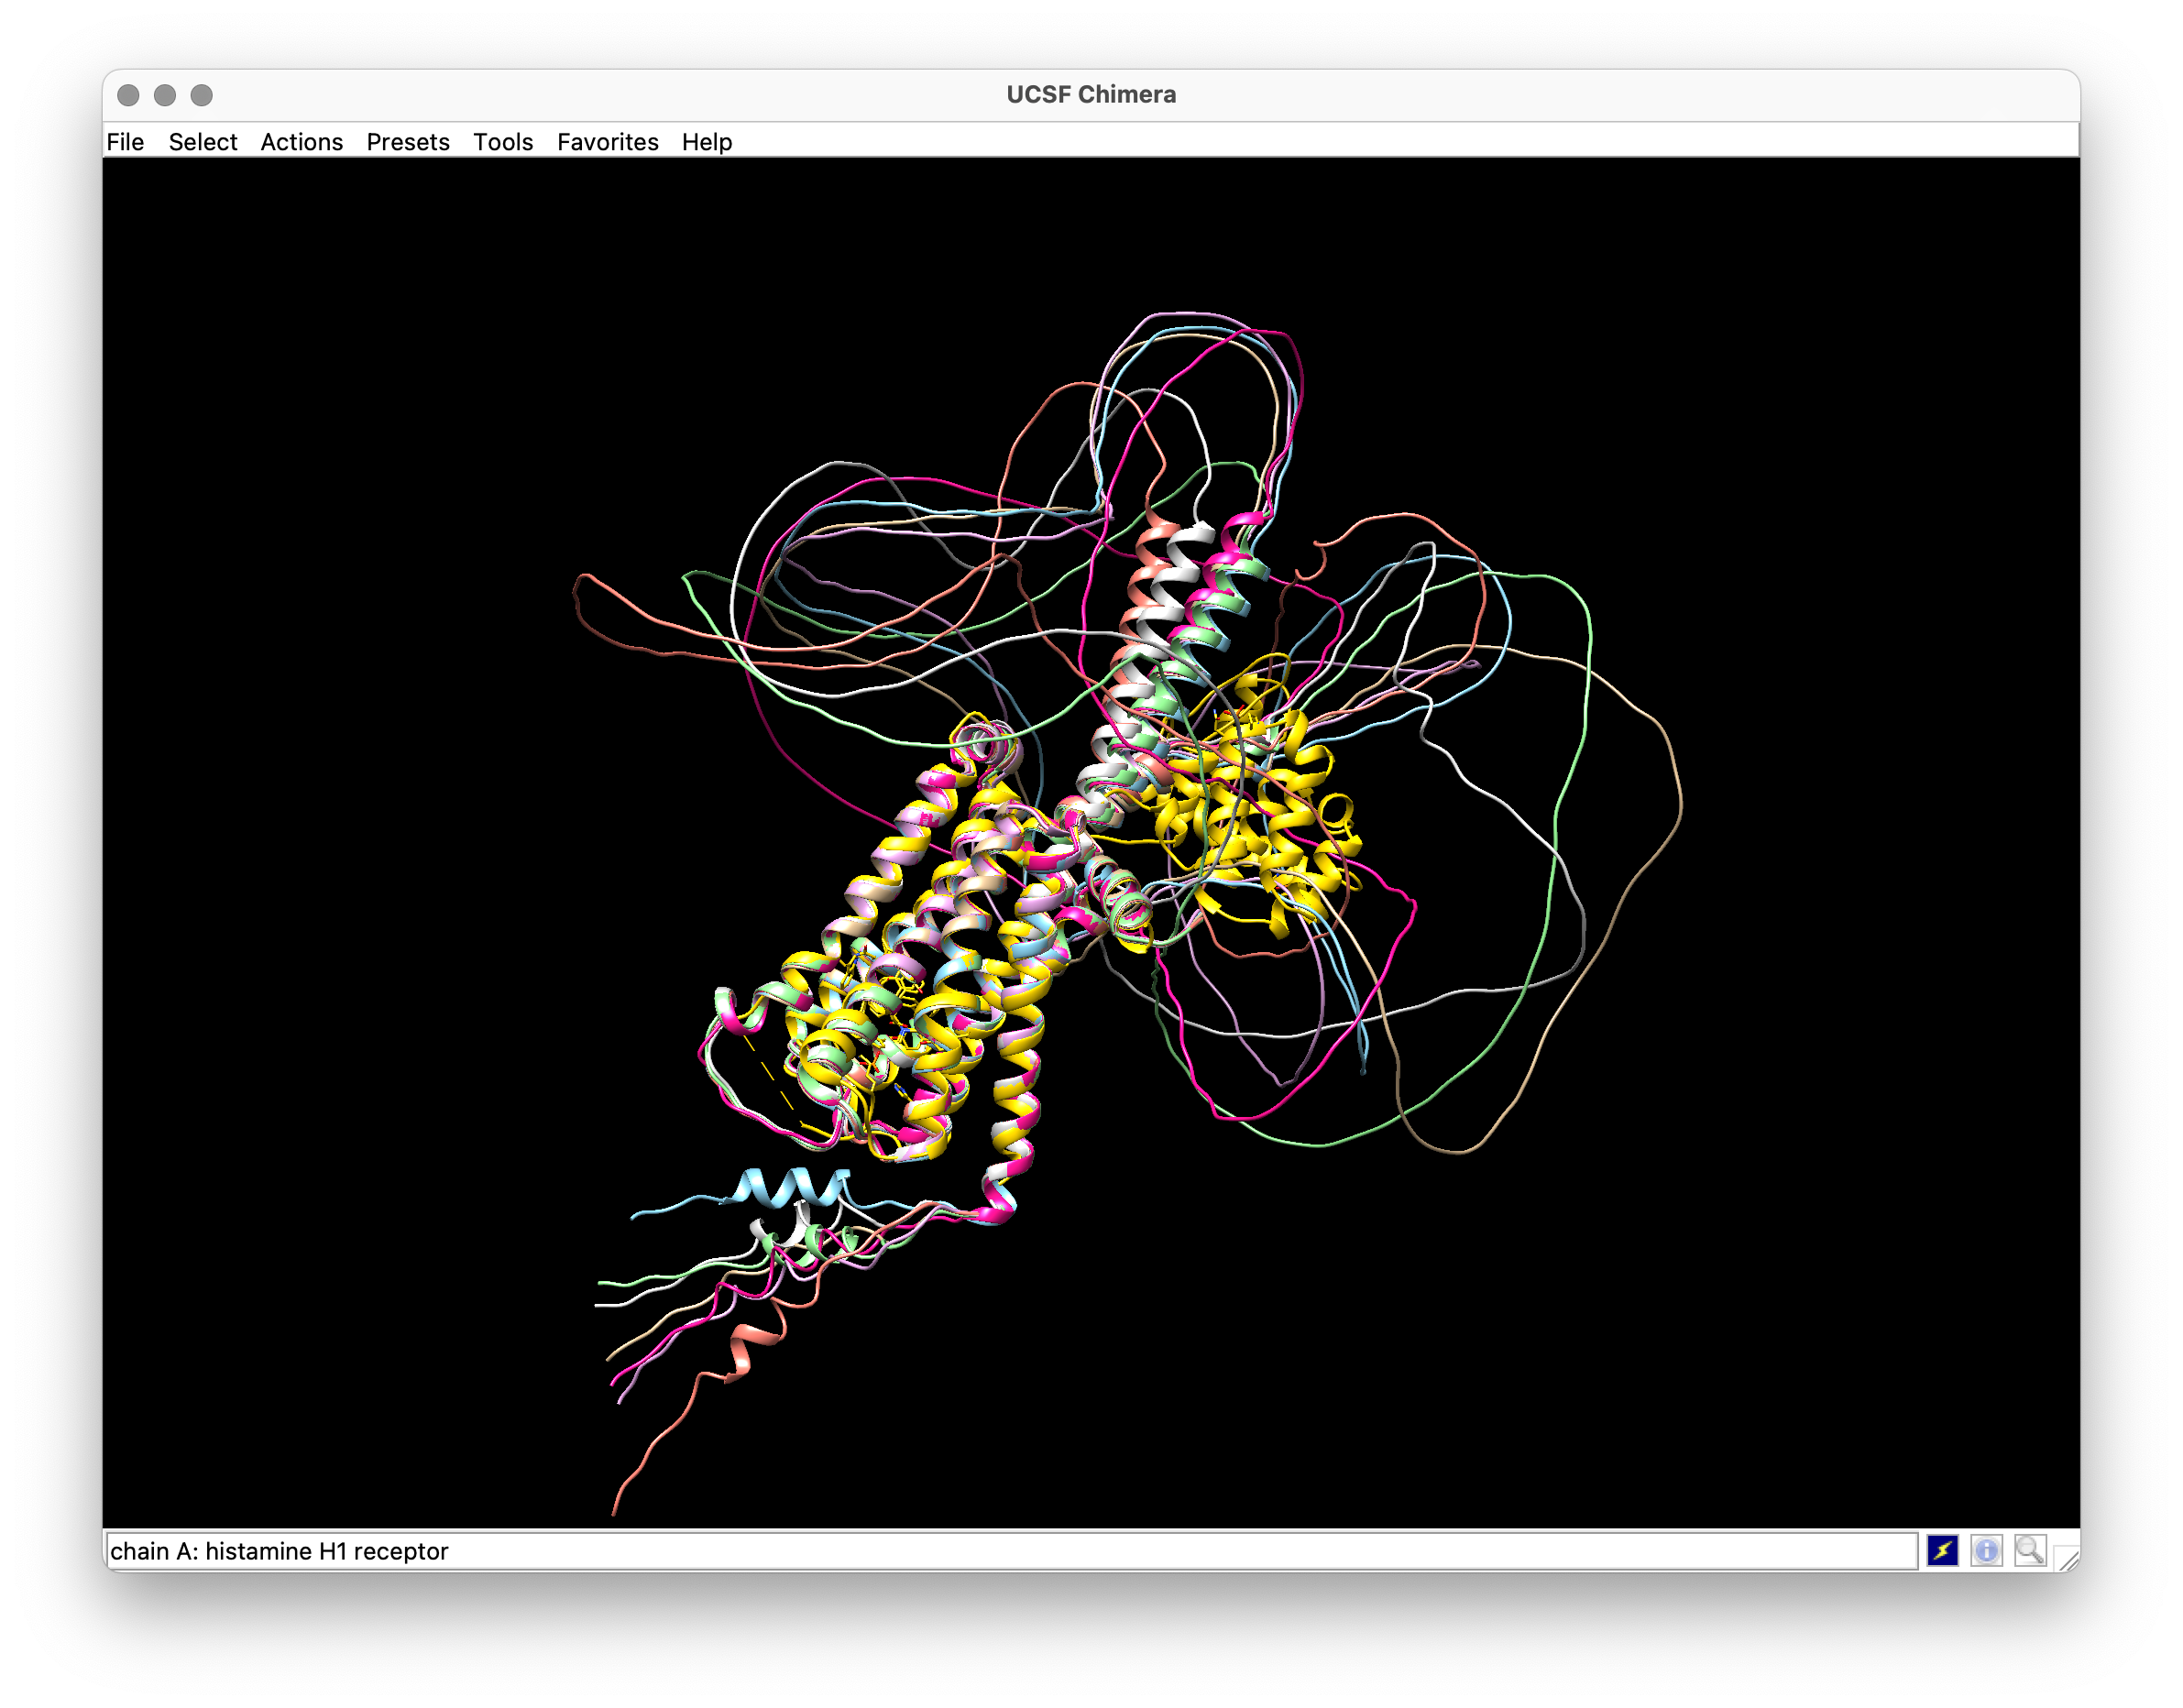
\includegraphics[width=0.8\textwidth]{CAA84380.1/_img/match maker results}
    \caption{Structural alignment results showing superimposed histamine structures.}
    \label{fig:histamine-alignment-results}
\end{figure}

\subsubsection{Sequence Conservation Analysis}\label{subsubsec:histamine-conservation}
The sequence alignment visualization (Figure \ref{fig:histamine-sequence-alignment}) revealed highly conserved regions, particularly in the core structural elements. The sequence identity matrix (Figure \ref{fig:histamine-sequence-identity}) showed identity values ranging from 63.05\% to 100\% between different species pairs.

\begin{figure}[H]
    \centering
    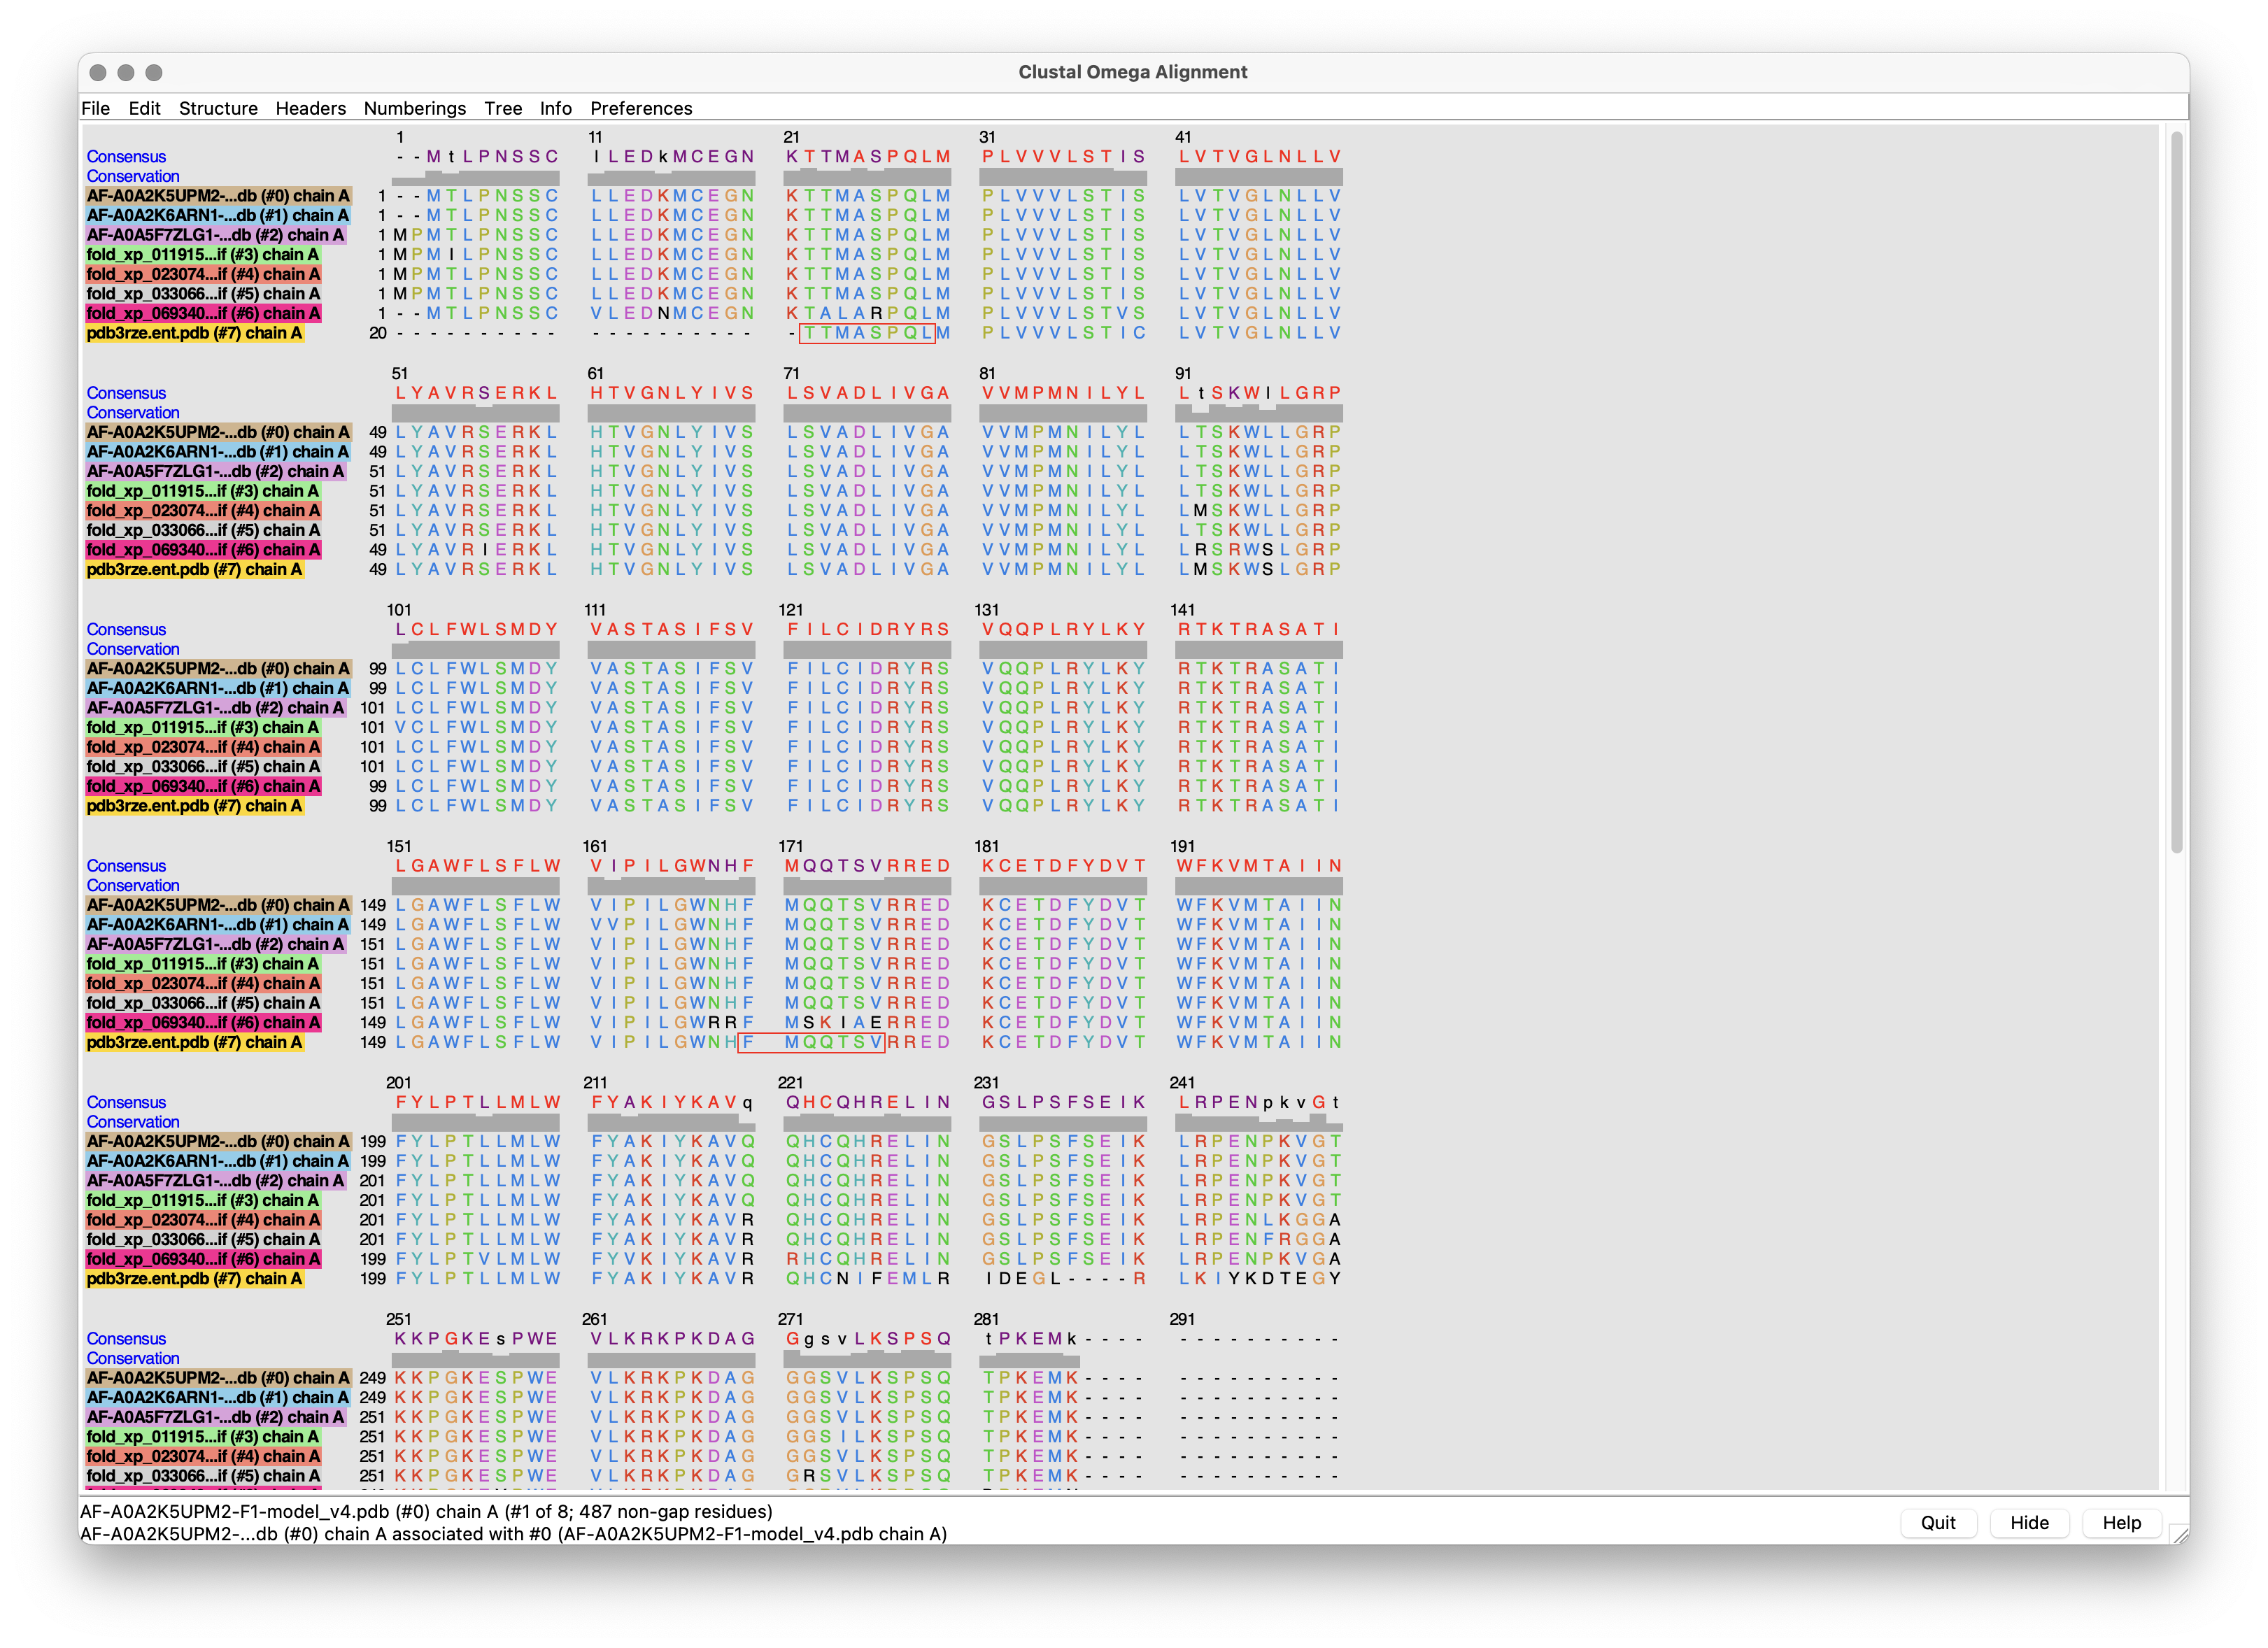
\includegraphics[width=0.8\textwidth]{CAA84380.1/_img/seq alignment results}
    \caption{Multiple sequence alignment of histamine proteins showing conservation patterns.}
    \label{fig:histamine-sequence-alignment}
\end{figure}

\begin{figure}[H]
    \centering
    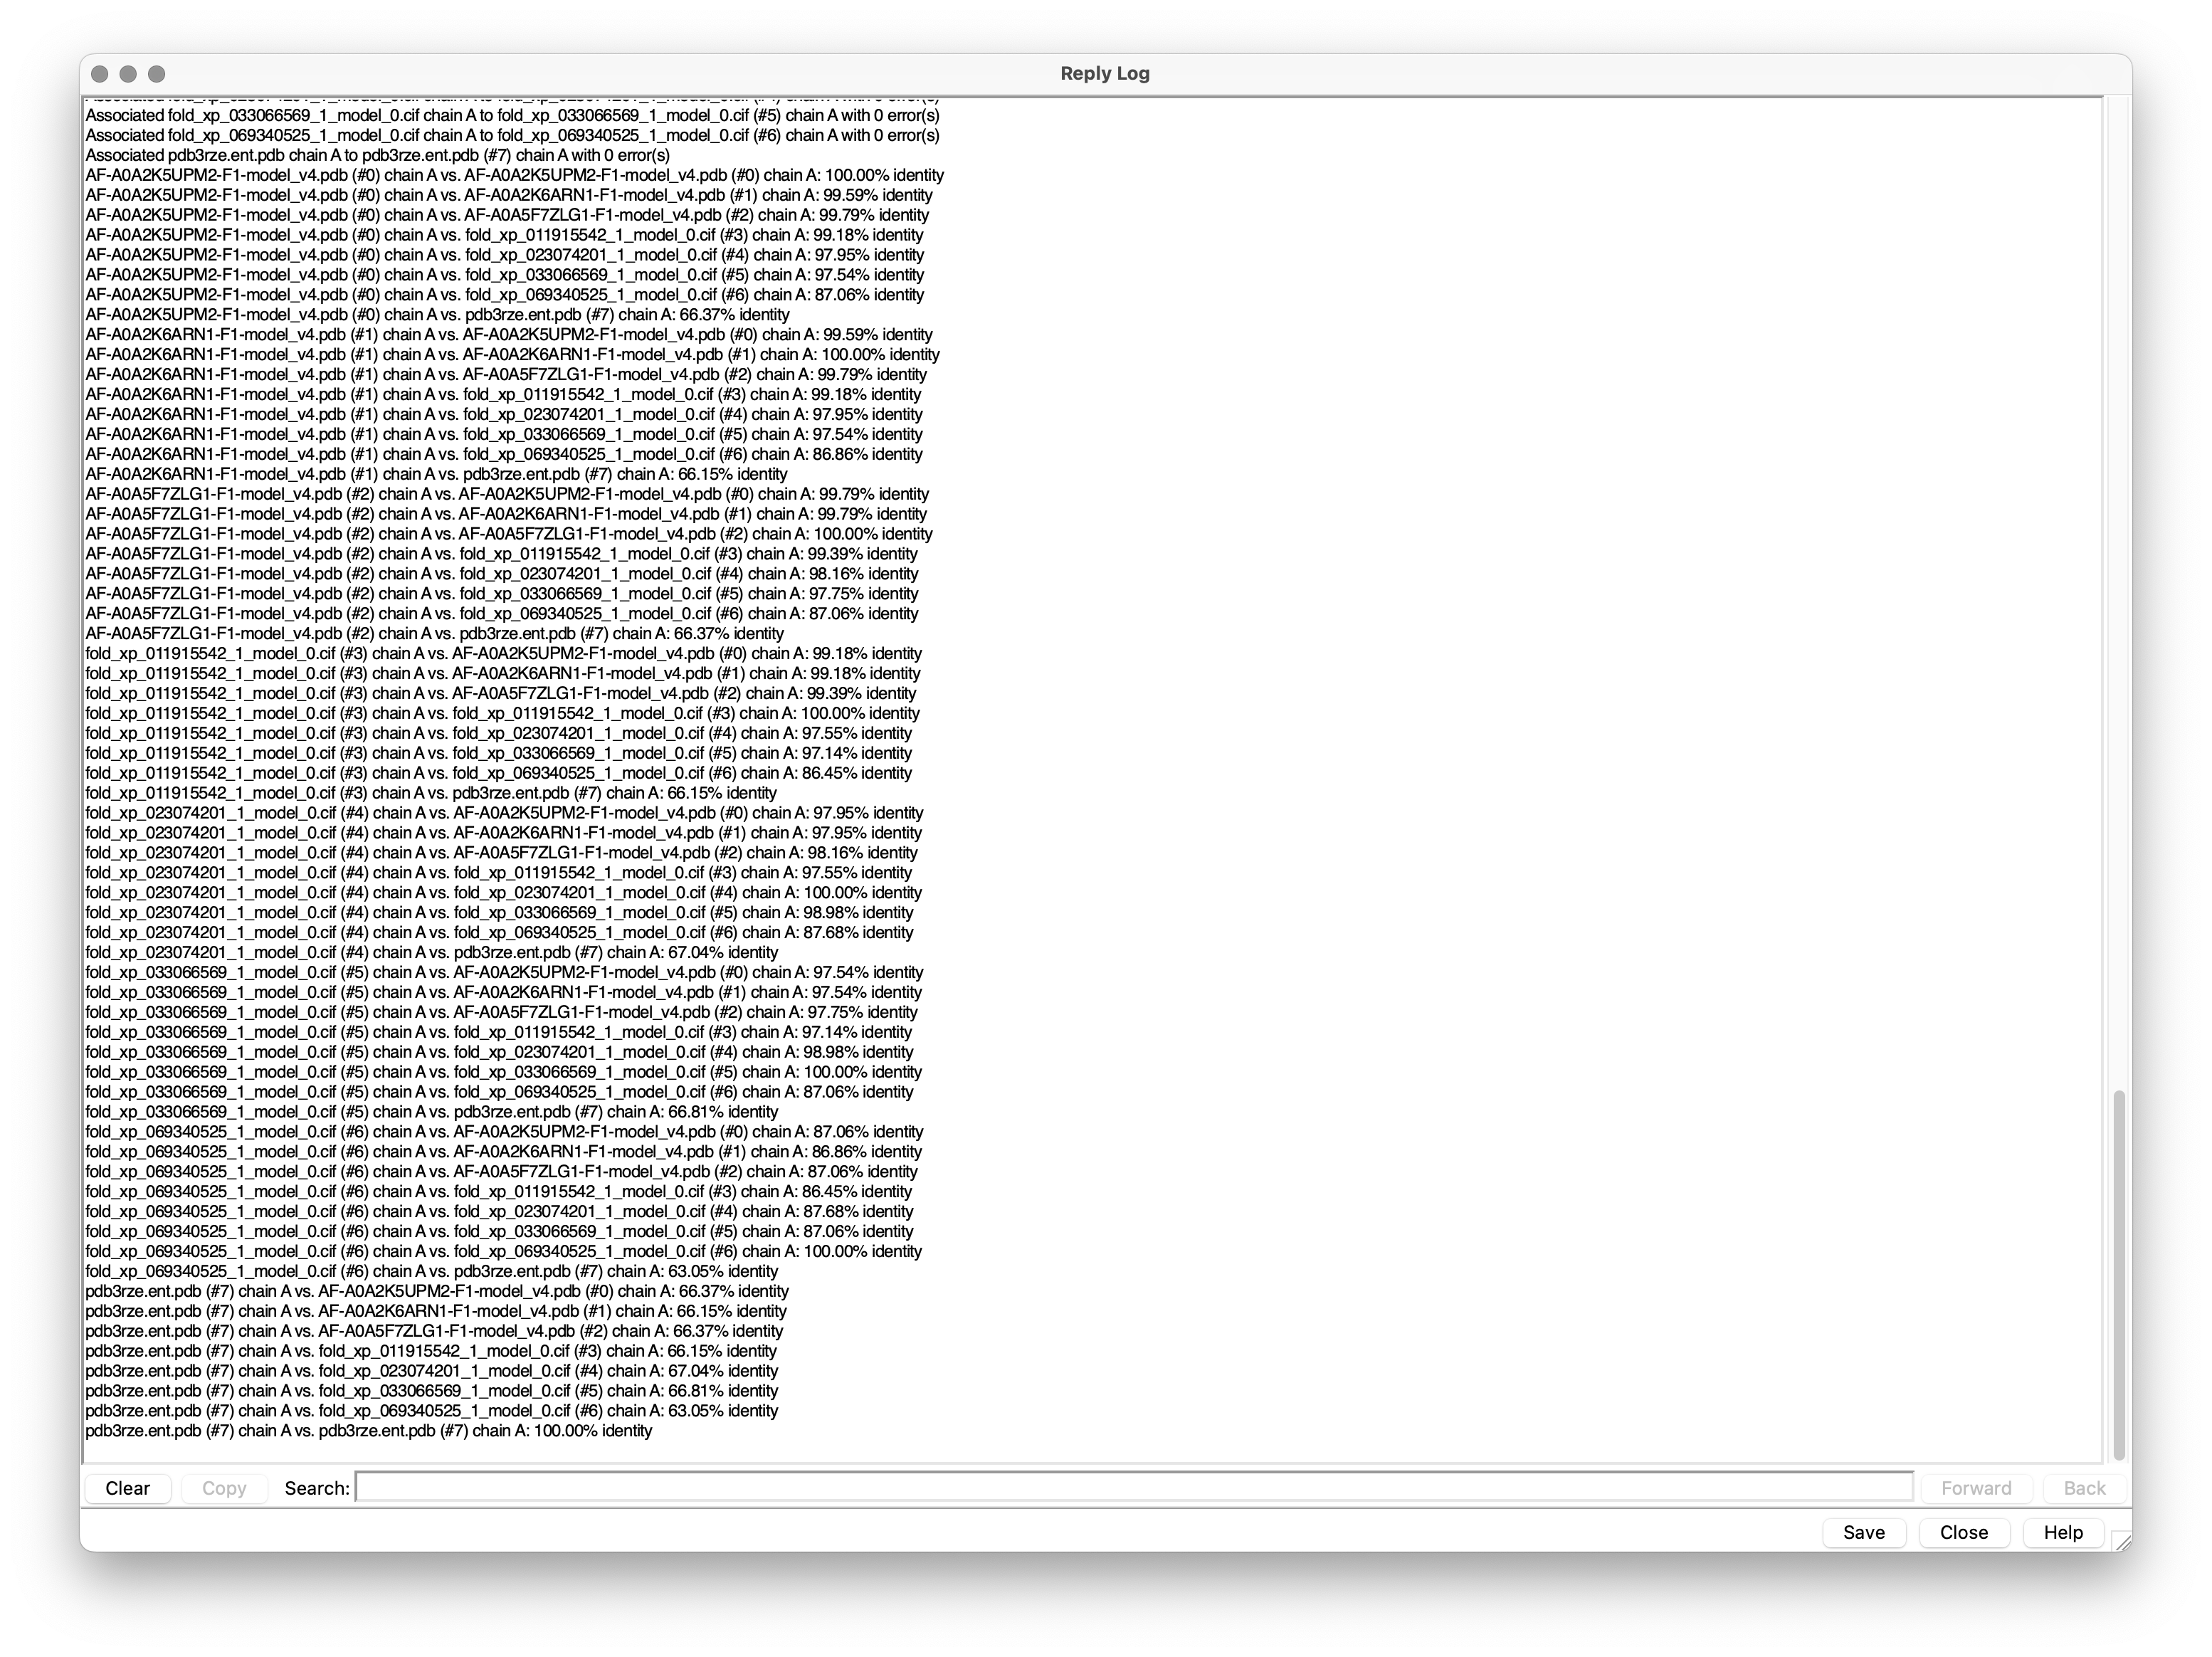
\includegraphics[width=0.8\textwidth]{CAA84380.1/_img/seq identity results}
    \caption{Sequence identity matrix showing pairwise comparisons between histamine structures.}
    \label{fig:histamine-sequence-identity}
\end{figure}

\subsubsection{Structure Conservation Visualization}\label{subsubsec:histamine-conservation-vis}
The conservation analysis was visualized using Chimera's built-in tools (Figure \ref{fig:histamine-conservation-render}), highlighting the structural elements that are most conserved across species.

\begin{figure}[H]
    \centering
    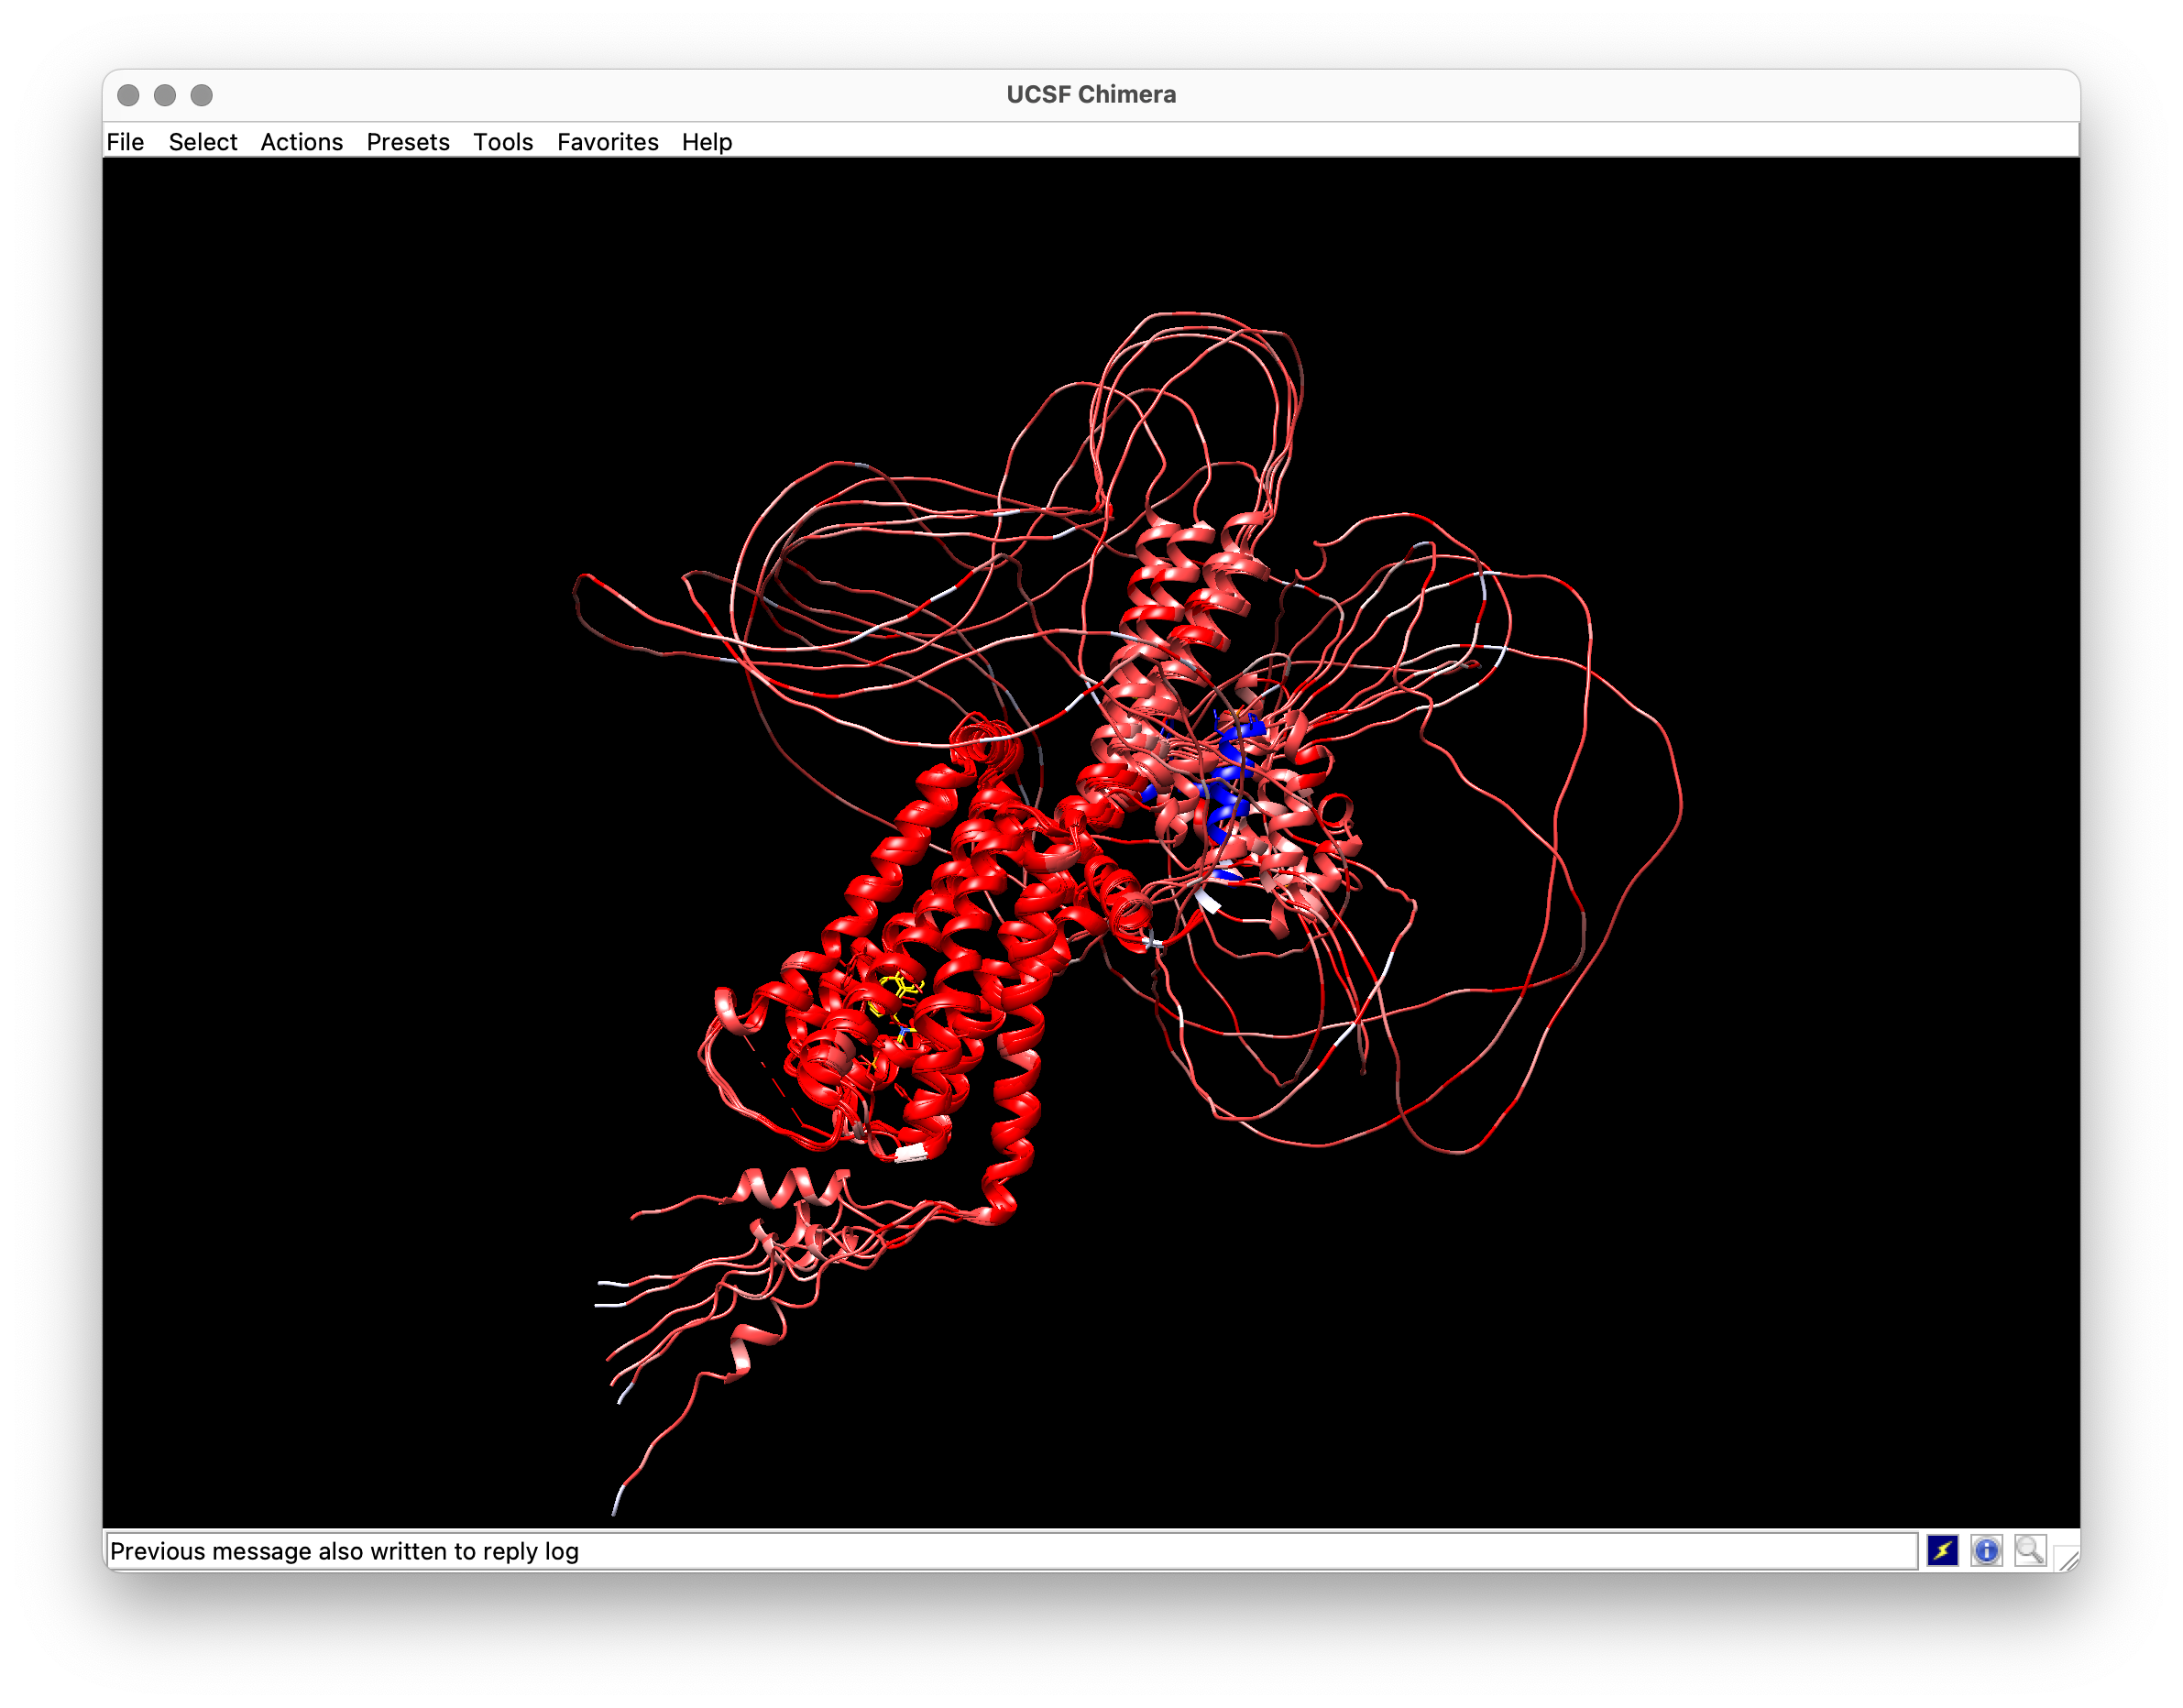
\includegraphics[width=0.8\textwidth]{CAA84380.1/_img/conservation render}
    \caption{Visualization of structural conservation across histamine proteins.}
    \label{fig:histamine-conservation-render}
\end{figure}

\subsubsection{Ensemble Analysis}\label{subsubsec:histamine-ensemble}
Finally, the Ensemble Match tool was attempted to compare multiple structures simultaneously. However, this resulted in an error due to unequal numbers of atoms in the structures (Figure \ref{fig:histamine-ensemble-match}).

\begin{figure}[H]
    \centering
    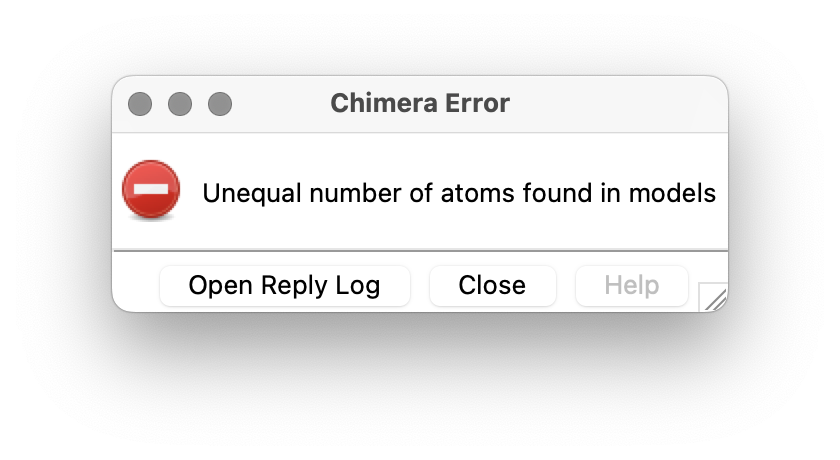
\includegraphics[width=0.8\textwidth]{CAA84380.1/_img/ensemble match}
    \caption{Ensemble Match Gives "Unequal number of atoms" error}
    \label{fig:histamine-ensemble-match}
\end{figure}

\subsubsection{Structural Comparison Conclusions}\label{subsubsec:histamine-conclusions}

Based on the sequence identity matrix and structural alignment results, the following key observations were made:

\paragraph{Most Similar Structures} The two most similar histamine H1 receptor structures were found between:
\begin{itemize}
    \item Macaca fascicularis (AF-A0A2K5UPM2) and Macaca nemestrina (AF-A0A2K6ARN1) receptors, showing 100\% sequence identity and identical structural features
    \item Macaca fascicularis (AF-A0A2K5UPM2) and Macaca mulatta (AF-A0A5F7ZLG1) receptors, with 99.79\% sequence identity and nearly identical structural arrangement
\end{itemize}

\paragraph{Most Different Structures} The greatest structural differences were observed between:
\begin{itemize}
    \item Human (pdb3rze) and Eulemur rufifrons (fold\_xp\_069340525) receptors, with sequence identity of 63.05\%, showing significant differences in both transmembrane and loop regions
    \item Eulemur rufifrons (fold\_xp\_069340525) and Trachypithecus francoisi (fold\_xp\_033066569) receptors, displaying considerable variations in their extracellular domains
\end{itemize}

\paragraph{Structure-Sequence Correlation} A detailed analysis revealed strong correlation between sequence and structural differences:
\begin{itemize}
    \item The seven-transmembrane helical core is well preserved across all species despite sequence variations
    \item The most significant structural differences appear in the extracellular and intracellular loop regions
    \item Species within the same genus (particularly Macaca species) maintain extremely high structural similarity ($>$97\% sequence identity)
    \item The experimentally determined human structure (X-ray diffraction, 3.10\AA{} resolution) shows some unique features compared to the predicted structures, particularly in loop regions
\end{itemize}

These findings demonstrate that while histamine H1 receptors show greater sequence diversity compared to insulin proteins, their core functional architecture remains highly conserved. This conservation pattern aligns with the receptor's crucial role in maintaining consistent signaling function across species, while allowing for species-specific adaptations in less critical regions.

\end{document}